\documentclass[UTF8,zihao=5]{ctexart}
\usepackage[a4paper,top=2.5cm,bottom=2.5cm,left=2.7cm,right=2.7cm]{geometry}
\usepackage{graphicx}
\usepackage{float}
\usepackage{booktabs}
\usepackage{array}
\usepackage{amsmath,amssymb,amsfonts}
\usepackage{hyperref}
\usepackage{xcolor}
\usepackage{listings}
\usepackage{caption}
\usepackage{subcaption}
\usepackage{fancyhdr}
\usepackage{enumitem}
\setmainfont{Times New Roman}
\hypersetup{colorlinks=true,linkcolor=black,citecolor=black,urlcolor=blue}
\setlength{\parindent}{2em}
\setlength{\parskip}{0em}
\setlength{\headheight}{15pt}
\setlength{\tabcolsep}{5pt}
\emergencystretch=2em
\linespread{1.24}
\pagestyle{fancy}
\fancyhf{}
\fancyhead[L]{信息安全技术期末课程报告}
\fancyhead[R]{MBRS 与 DWSF 复现对比}
\fancyfoot[C]{\thepage}
\lstset{basicstyle=\small\ttfamily,breaklines=true,breakatwhitespace=false,frame=single,columns=fullflexible,keepspaces=true,showstringspaces=false,backgroundcolor=\color{gray!6}}
\renewcommand{\figurename}{图}
\renewcommand{\tablename}{表}
\begin{document}
\begin{titlepage}
\centering
\vspace*{1.5cm}
{\zihao{1}\bfseries 信息安全技术期末课程报告\par}
\vspace{1.2cm}
{\zihao{2}\bfseries 基于深度学习的鲁棒图像水印方法复现与对比：MBRS 与 DWSF\par}
\vspace{2.0cm}
\begin{tabular}{rl}
\textbf{选题方向：} & 方向 2：复现两篇同领域 CCF-B 以上论文并对比优缺点\\[0.35em]
\textbf{研究领域：} & 数字水印、深度学习图像水印、鲁棒盲水印\\[0.35em]
\textbf{组员：} & 梁力航、苟一霏\\[0.35em]
\textbf{提交日期：} & 2025 年 7 月\\
\end{tabular}
\vfill
\begin{flushleft}
\textbf{复现论文：}
\begin{enumerate}[leftmargin=2em]
\item Zhaoyang Jia, Han Fang, Weiming Zhang. \emph{MBRS: Enhancing Robustness of DNN-based Watermarking by Mini-Batch of Real and Simulated JPEG Compression}. ACM MM 2021.
\item Hengchang Guo, Qilong Zhang, Junwei Luo, Feng Guo, Wenbin Zhang, Xiaodong Su, Minglei Li. \emph{Practical Deep Dispersed Watermarking with Synchronization and Fusion}. ACM MM 2023.
\end{enumerate}
\end{flushleft}
\end{titlepage}
\begin{abstract}

数字水印技术是信息安全领域中面向版权保护、内容溯源和泄露追踪的重要技术。传统水印方法通常依赖 DCT、DWT 等人工设计的频域特征，在特定攻击下可以取得较好效果，但对复杂图像内容、组合失真和真实应用场景的适应性有限。随着深度学习的发展，基于编码器-噪声层-解码器的端到端图像水印方法逐渐成为鲁棒水印研究的重要方向。本文选择 ACM MM 2021 论文 MBRS 与 ACM MM 2023 论文 DWSF 作为复现对象。两者均属于深度学习鲁棒图像水印方法，但研究重点不同：MBRS 主要针对 JPEG 压缩这一非可微但实际高频出现的攻击，提出真实 JPEG、模拟 JPEG 与无噪声层混合的小批次训练策略；DWSF 则面向任意分辨率图像和复杂几何攻击，提出分散嵌入、水印同步和消息融合机制。

在复现过程中，我们基于两篇论文公开代码整理了统一的训练、评估和可视化流程，并在本地 Apple M4 + MPS 环境下完成轻量化复现实验。实验使用 128×128 图像块、随机二进制消息以及 PSNR、SSIM、BER 等标准评价指标，对两种方法在无攻击、JPEG 压缩、高斯模糊、高斯噪声、裁剪和亮度变化等多种攻击下的表现进行了对比。实验结果表明，MBRS 在无攻击图像质量和轻度 JPEG 压缩下表现更优，Clean 条件下 PSNR 达到 33.8 dB，BER 为 0；DWSF 参数量约为 MBRS 的五分之一，也能在 Clean 条件下实现 BER 为 0，并在部分亮度变化场景下表现更好。对于强压缩、强模糊和裁剪等更高强度扰动，两种模型呈现出不同的鲁棒性变化趋势，为分析水印嵌入策略和攻击适应性提供了实验依据。本文进一步分析了两种方法的结构差异、鲁棒性来源、复现结果和实际应用取舍，并总结了本次复现实验对深度水印系统设计的启示。


\end{abstract}
\clearpage
\tableofcontents
\clearpage
\section{背景与动机}

\subsection{数字水印与信息安全需求}

数字内容在互联网平台、社交媒体、云存储和生成式人工智能系统中被快速复制和传播。图像、视频、音频等多媒体内容一旦脱离原始发布环境，就容易出现未经授权转载、篡改传播、版权归属难以确认等问题。数字水印技术的目标是在不明显破坏内容质量的前提下，将身份标识、版权信息或追踪码嵌入到多媒体内容中，并在内容经历压缩、裁剪、噪声、滤波、亮度变化等处理后仍然能够恢复水印信息。因此，一个实用的图像水印系统通常需要同时满足三个条件：不可感知性、鲁棒性和可提取性。

不可感知性要求水印嵌入后图像与原图在视觉上尽量一致，避免影响正常使用。鲁棒性要求水印在常见图像处理甚至恶意攻击后仍能被检测或提取。可提取性则要求解码端能够准确恢复嵌入的比特序列。三者之间存在明显矛盾：嵌入越强，通常越容易被提取，也越容易造成视觉失真；嵌入越弱，图像质量越好，但抗攻击能力可能下降。因此，数字水印问题本质上是一个安全性、鲁棒性与图像质量之间的权衡问题。

传统图像水印方法通常在空域或频域中嵌入水印。例如，最低有效位方法实现简单，但容易被统计检测和图像处理破坏；DCT 和 DWT 频域方法更适合应对压缩和滤波，但通常依赖人工设计规则，对复杂内容自适应能力不足。深度学习方法通过神经网络自动学习嵌入位置和特征表达，使编码器能够根据图像内容生成水印图像，使解码器能够从受扰动图像中恢复消息。这种端到端训练方式为鲁棒水印提供了新的技术路线。

\subsection{深度水印的基本框架}

当前许多深度图像水印方法都采用类似自动编码器的框架：编码器接收原始图像和待嵌入消息，输出水印图像；噪声层模拟 JPEG 压缩、裁剪、模糊、噪声等攻击；解码器从噪声层输出图像中恢复消息；判别器或图像损失用于约束水印图像与原图的视觉相似性。训练时，编码器和解码器需要在图像失真损失、消息恢复损失和对抗损失之间取得平衡。

这种框架的关键难点在于噪声层的设计。如果攻击可微，例如高斯噪声、模糊、亮度变化等，可以直接嵌入计算图中进行反向传播；但 JPEG 压缩包含量化、舍入等非可微操作，直接用于端到端训练会阻断梯度。另一方面，真实场景中 JPEG 压缩极其常见，许多图像在平台上传、转发和存储过程中都会被重新压缩。因此，如何让深度水印模型在训练时学习 JPEG 鲁棒性，是 MBRS 重点解决的问题。

除了压缩攻击，实际图像还可能经历旋转、缩放、裁剪、透视变换、拼接、局部遮挡等几何扰动。几何攻击不仅改变像素值，还会破坏编码器和解码器之间的空间对应关系。固定输入分辨率的小图块水印方法在高分辨率实际图像上也存在应用不便的问题。DWSF 正是针对这一类实际问题，提出将水印分散嵌入多个图像块，并在解码阶段先定位水印块，再进行消息融合。

\subsection{选题动机}

我们选择 MBRS 和 DWSF 作为复现对象，主要有两点原因。

第一，两篇论文都属于信息安全与数字水印方向，均发表在 ACM MM，满足课程对 CCF-B 以上论文的要求。第二，两者方法具有明显继承关系和对比价值：MBRS 代表较典型的固定尺寸端到端深度鲁棒水印框架，重点解决 JPEG 压缩；DWSF 则进一步面向真实应用中的任意分辨率和几何扰动，尝试把局部水印、同步定位和消息融合结合起来。

通过本次复现，我们希望回答以下问题：一是深度水印方法在轻量化复现实验中能否同时保持图像质量和消息提取准确率；二是 MBRS 和 DWSF 的鲁棒性差异主要体现在哪些攻击类型上；三是参数量、消息长度、嵌入策略和攻击适应性之间存在怎样的取舍；四是这些方法在课程实验环境和实际部署中分别适合怎样的应用范围。


\section{论文方案介绍与方法关系}

\subsection{MBRS 方法原理}

MBRS 的全称为 Mini-Batch of Real and Simulated JPEG Compression，其核心目标是增强深度水印模型对 JPEG 压缩的鲁棒性。论文指出，许多基于 DNN 的水印方法可以通过可微噪声层学习抗噪声、抗模糊等能力，但 JPEG 压缩中量化操作不可微，训练时如果只使用近似 JPEG，模型容易偏向模拟分布；如果直接使用真实 JPEG，又无法稳定反向传播。MBRS 的解决思路是在不同 mini-batch 中随机选择真实 JPEG、模拟 JPEG 或无噪声层作为训练扰动，使模型既接触真实压缩效果，又保留可微近似提供的梯度信息。

更具体地说，设原始图像为 \(I \in \mathbb{R}^{H \times W \times 3}\)，待嵌入消息为二进制向量 \(m \in \{0,1\}^{L}\)。编码器 \(E_{\theta}\) 将图像和消息映射为水印图像：

\[
I_w = E_{\theta}(I, m)
\]

噪声层 \(N(\cdot)\) 模拟图像在真实传播过程中的失真，得到受扰动图像：

\[
I_n = N(I_w)
\]

解码器 \(D_{\phi}\) 从受扰动图像中恢复消息：

\[
\hat{m} = D_{\phi}(I_n)
\]

训练目标是让 \(I_w\) 与 \(I\) 尽量接近，同时让 \(\hat{m}\) 与 \(m\) 尽量一致。MBRS 还引入判别器 \(C_{\psi}\)，使水印图像在判别器看来更接近真实 cover image。根据代码中的训练逻辑，编码器-解码器的总损失可以概括为：

\[
\mathcal{L}_{G}
= \lambda_{adv}\mathcal{L}_{adv}
+ \lambda_{img}\mathcal{L}_{img}
+ \lambda_{msg}\mathcal{L}_{msg}
\]

其中：

\[
\mathcal{L}_{img}=\|I_w-I\|_2^2,\qquad
\mathcal{L}_{msg}=\|\hat{m}-m\|_2^2
\]

\[
\mathcal{L}_{adv}=\mathrm{BCE}(C_{\psi}(I_w),1)
\]

\(\mathcal{L}_{img}\) 约束不可感知性，\(\mathcal{L}_{msg}\) 约束消息恢复准确率，\(\mathcal{L}_{adv}\) 通过对抗学习提升水印图像自然性。判别器本身则学习区分原图和水印图像，其损失可写为：

\[
\mathcal{L}_{C}
=\mathrm{BCE}(C_{\psi}(I),1)
+\mathrm{BCE}(C_{\psi}(I_w),0)
\]

这个目标函数体现了深度水印的核心权衡：图像越接近原图，水印越隐蔽；消息越容易恢复，水印越鲁棒；判别器约束则进一步提升视觉自然性。

MBRS 最关键的设计是 mini-batch 级别的 JPEG 噪声选择。普通可微噪声层可以直接反向传播，但真实 JPEG 中存在量化和取整操作，梯度不稳定。MBRS 不在每张图像上混合所有噪声，而是在每个 mini-batch 中选择一种噪声路径：

\[
N \in \{N_{realJPEG}, N_{simJPEG}, N_{identity}\}
\]

其中 \(N_{realJPEG}\) 表示真实 JPEG 压缩，\(N_{simJPEG}\) 表示可微或近似可微的模拟 JPEG，\(N_{identity}\) 表示无压缩路径。这样做的直观含义是：真实 JPEG 让模型看到真实压缩后的图像分布，模拟 JPEG 提供可学习的梯度，无噪声路径保持 clean 图像下的消息恢复能力。三者结合后，模型不会只适应某一种理想化攻击，而是能够在压缩与无压缩场景之间取得平衡。

在网络结构上，MBRS 还引入 Squeeze-and-Excitation 模块和 message processor。SE 模块通过通道注意力机制提升特征表达能力，使网络能够更有效地选择适合嵌入水印的信息通道；message processor 将原始二进制消息扩展成更适合与图像特征融合的高维表示，有助于提高嵌入和解码稳定性。论文还讨论了 diffusion block 用于增强裁剪攻击下的鲁棒性。

从代码结构看，MBRS 编码器首先对图像做卷积和 SE 特征提取；同时将消息 reshape 成小的消息图，再经过 ExpandNet 和 SE 模块扩展到与图像特征相同的空间尺度；随后将图像特征和消息特征拼接，并通过卷积层生成水印图像。这个过程可以理解为把一维消息 \(m\) 转换成空间特征图 \(F_m\)，再与图像特征 \(F_I\) 融合：

\[
F_I=f_I(I),\qquad F_m=f_m(m),\qquad I_w=f_{out}([F_I,F_m,I])
\]

其中 \([\,\cdot\,]\) 表示通道拼接。相比直接把比特拼接到图像通道上，message processor 能让消息在空间维度上扩散，更适合卷积网络学习稳定的嵌入模式。

从安全应用角度看，MBRS 的优势是针对性强，尤其适合图像在网络平台传播时常见的 JPEG 压缩场景。由于其主要围绕固定尺寸图像块进行建模，后续也可以与多块嵌入、几何同步等机制结合，进一步扩展到大尺寸图像和组合攻击场景。

\subsection{DWSF 方法原理}

DWSF 的全称为 Deep Dispersed Watermarking with Synchronization and Fusion，目标是构建更实用的盲水印框架。论文认为，已有深度水印工作往往集中在固定低分辨率图像上，并主要验证非几何攻击，例如 JPEG 压缩和高斯噪声；但真实应用中图像通常是高分辨率的，并可能经历旋转、缩放、裁剪等几何攻击。为解决这些问题，DWSF 提出了三个关键组件：分散嵌入、水印同步和消息融合。

\begin{figure}[H]
\centering
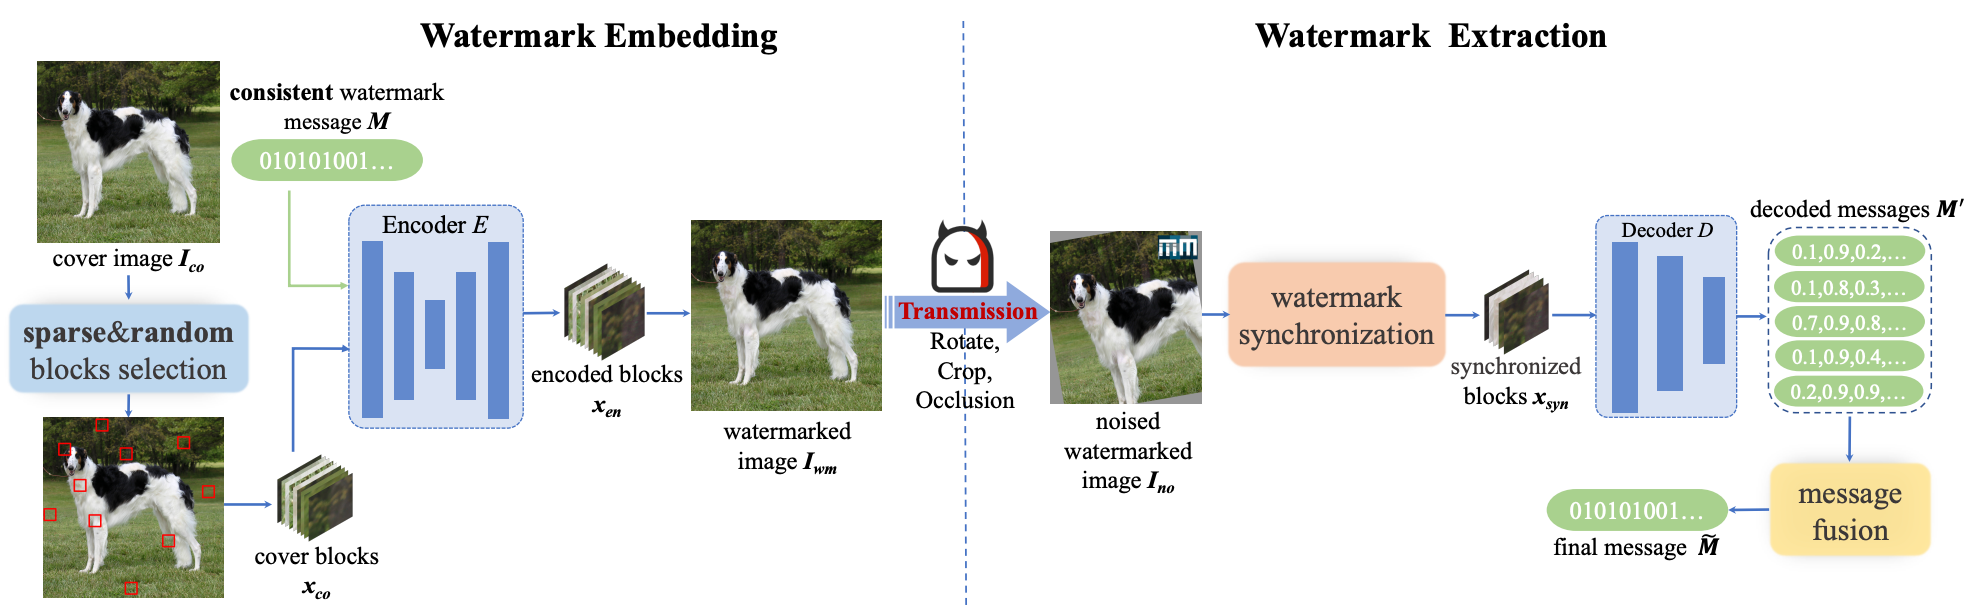
\includegraphics[width=0.92\textwidth]{../code/DWSF/IMG/framework.png}
\caption{DWSF 官方框架图。 DWSF 将任意分辨率图像划分为多个局部候选块，在若干图像块中分散嵌入相同消息；提取阶段先通过同步模块定位水印区域，再由解码器和融合策略恢复最终消息。}
\end{figure}

分散嵌入指的是在任意分辨率 cover image 中随机选择多个固定大小的图像块，并在这些图像块中嵌入相同水印消息。这样做有两个好处：一方面，模型仍然可以使用固定尺寸编码器处理局部块，避免直接训练高分辨率大模型；另一方面，同一消息被嵌入多个位置后，即使部分区域被裁剪、遮挡或破坏，仍可能从其他区域恢复消息。

用符号表示，设任意分辨率图像为 \(I\)，从中选出 \(K\) 个图像块：

\[
\{P_1,P_2,\ldots,P_K\}=\mathrm{SelectBlocks}(I)
\]

每个图像块都嵌入同一条消息 \(m\)：

\[
P_i^w = E_{\theta}(P_i,m),\quad i=1,\ldots,K
\]

再将这些水印块放回原图，得到完整水印图像：

\[
I_w=\mathrm{Merge}(I,\{P_i^w\}_{i=1}^{K})
\]

这种分散嵌入本质上是一种空间冗余策略。单个水印块可能受到裁剪、遮挡或局部退化影响，但多个块同时携带相同消息，可以显著提升系统层面的恢复机会。

水印同步模块负责在受攻击图像中定位并校正水印块。几何攻击会改变水印块的位置和形状，如果直接将整图或错误图块输入解码器，消息恢复会失败。DWSF 使用类似分割模型的同步网络检测水印区域，并对候选区域进行对齐或修正，使后续解码器能够处理更接近训练分布的局部块。

同步阶段可以抽象为：

\[
\{\tilde{P}_1,\tilde{P}_2,\ldots,\tilde{P}_T\}
=S_{\omega}(I_a)
\]

其中 \(I_a\) 是经历攻击后的水印图像，\(S_{\omega}\) 是同步网络，输出一组候选水印块。随后解码器分别对这些候选块进行消息估计：

\[
\hat{m}_t=D_{\phi}(\tilde{P}_t),\quad t=1,\ldots,T
\]

消息融合策略用于整合多个水印块的解码结果。由于同一消息被嵌入多个块，不同块在攻击后质量不同，解码结果可靠性也不同。DWSF 根据消息之间的相似性或置信度进行融合，以得到最终更可靠的消息估计。与单块解码相比，融合机制可以降低局部失败对整体提取结果的影响。

融合可以理解为对多个候选解码结果进行加权投票：

\[
\hat{m}=\mathrm{Fusion}(\hat{m}_1,\hat{m}_2,\ldots,\hat{m}_T)
\]

若使用相似度或置信度权重 \(w_t\)，则可写成：

\[
\hat{m}=\mathbb{I}\left(\sum_{t=1}^{T}w_t\hat{m}_t \geq \tau \right)
\]

其中 \(\tau\) 是判定阈值，\(\mathbb{I}(\cdot)\) 表示逐比特阈值化。这个公式表达的是 DWSF 的核心思想：不依赖单个局部区域的一次解码结果，而是通过多个区域之间的一致性得到更可靠的最终消息。

DWSF 的编码器-解码器训练目标与 MBRS 类似，也需要同时优化图像质量、消息恢复和判别器约束。代码中编码损失结合了 MSE 和 MS-SSIM，可概括为：

\[
\mathcal{L}_{enc}
=\mathcal{L}_{MSE}(I_w,I)
+\alpha\mathcal{L}_{MS\text{-}SSIM}(I_w,I)
\]

\[
\mathcal{L}_{dec}=\|\hat{m}-m\|_2^2
\]

\[
\mathcal{L}_{total}
=\lambda_{adv}\mathcal{L}_{adv}
+\lambda_{enc}\mathcal{L}_{enc}
+\lambda_{dec}\mathcal{L}_{dec}
\]

其中 MS-SSIM 更关注结构相似性，有助于约束水印图像在感知层面的质量；解码损失保证消息提取准确；对抗损失则用于提升水印图像自然性。

DWSF 的优势在于更贴近实际应用：它支持任意分辨率输入，考虑几何扰动，并通过冗余嵌入提升鲁棒性。与 MBRS 相比，DWSF 的系统链路更完整，除编码器-解码器外还包含同步定位与融合模块，因此更适合讨论从算法模型走向实际水印系统时的工程设计。

\subsection{两种方案的关系与差异}

MBRS 和 DWSF 都属于深度鲁棒盲水印方法，都使用编码器-解码器结构学习水印嵌入与提取。二者的共同点包括：使用神经网络替代人工特征设计；通过噪声层模拟攻击；使用 PSNR、SSIM、BER 等指标评价图像质量和消息恢复效果；追求水印不可见与攻击后可恢复之间的平衡。

二者差异主要体现在研究目标和系统层级上。MBRS 关注“如何让固定尺寸深度水印模型更好地抵抗 JPEG 压缩”，属于对训练噪声层和网络结构的改进；DWSF 关注“如何让深度水印系统适应实际任意分辨率和几何攻击场景”，属于对整体水印应用流程的扩展。可以认为，MBRS 更偏向鲁棒训练策略，DWSF 更偏向实际系统设计。

从嵌入方式看，MBRS 在给定图像块中直接嵌入消息，输出同尺寸水印图像；DWSF 在大图中选择多个块分散嵌入相同消息。前者结构较简洁，训练和推理链路短；后者冗余度更高，抗局部破坏潜力更强。从攻击适应性看，MBRS 对 JPEG 压缩有明确优化目标；DWSF 对几何攻击、组合攻击和高分辨率图像更有设计优势。从复现难度看，MBRS 的编码器-解码器复现较直接；DWSF 完整复现需要额外同步模块和消息融合流程，实验复杂度更高。

\begin{figure}[H]
\centering
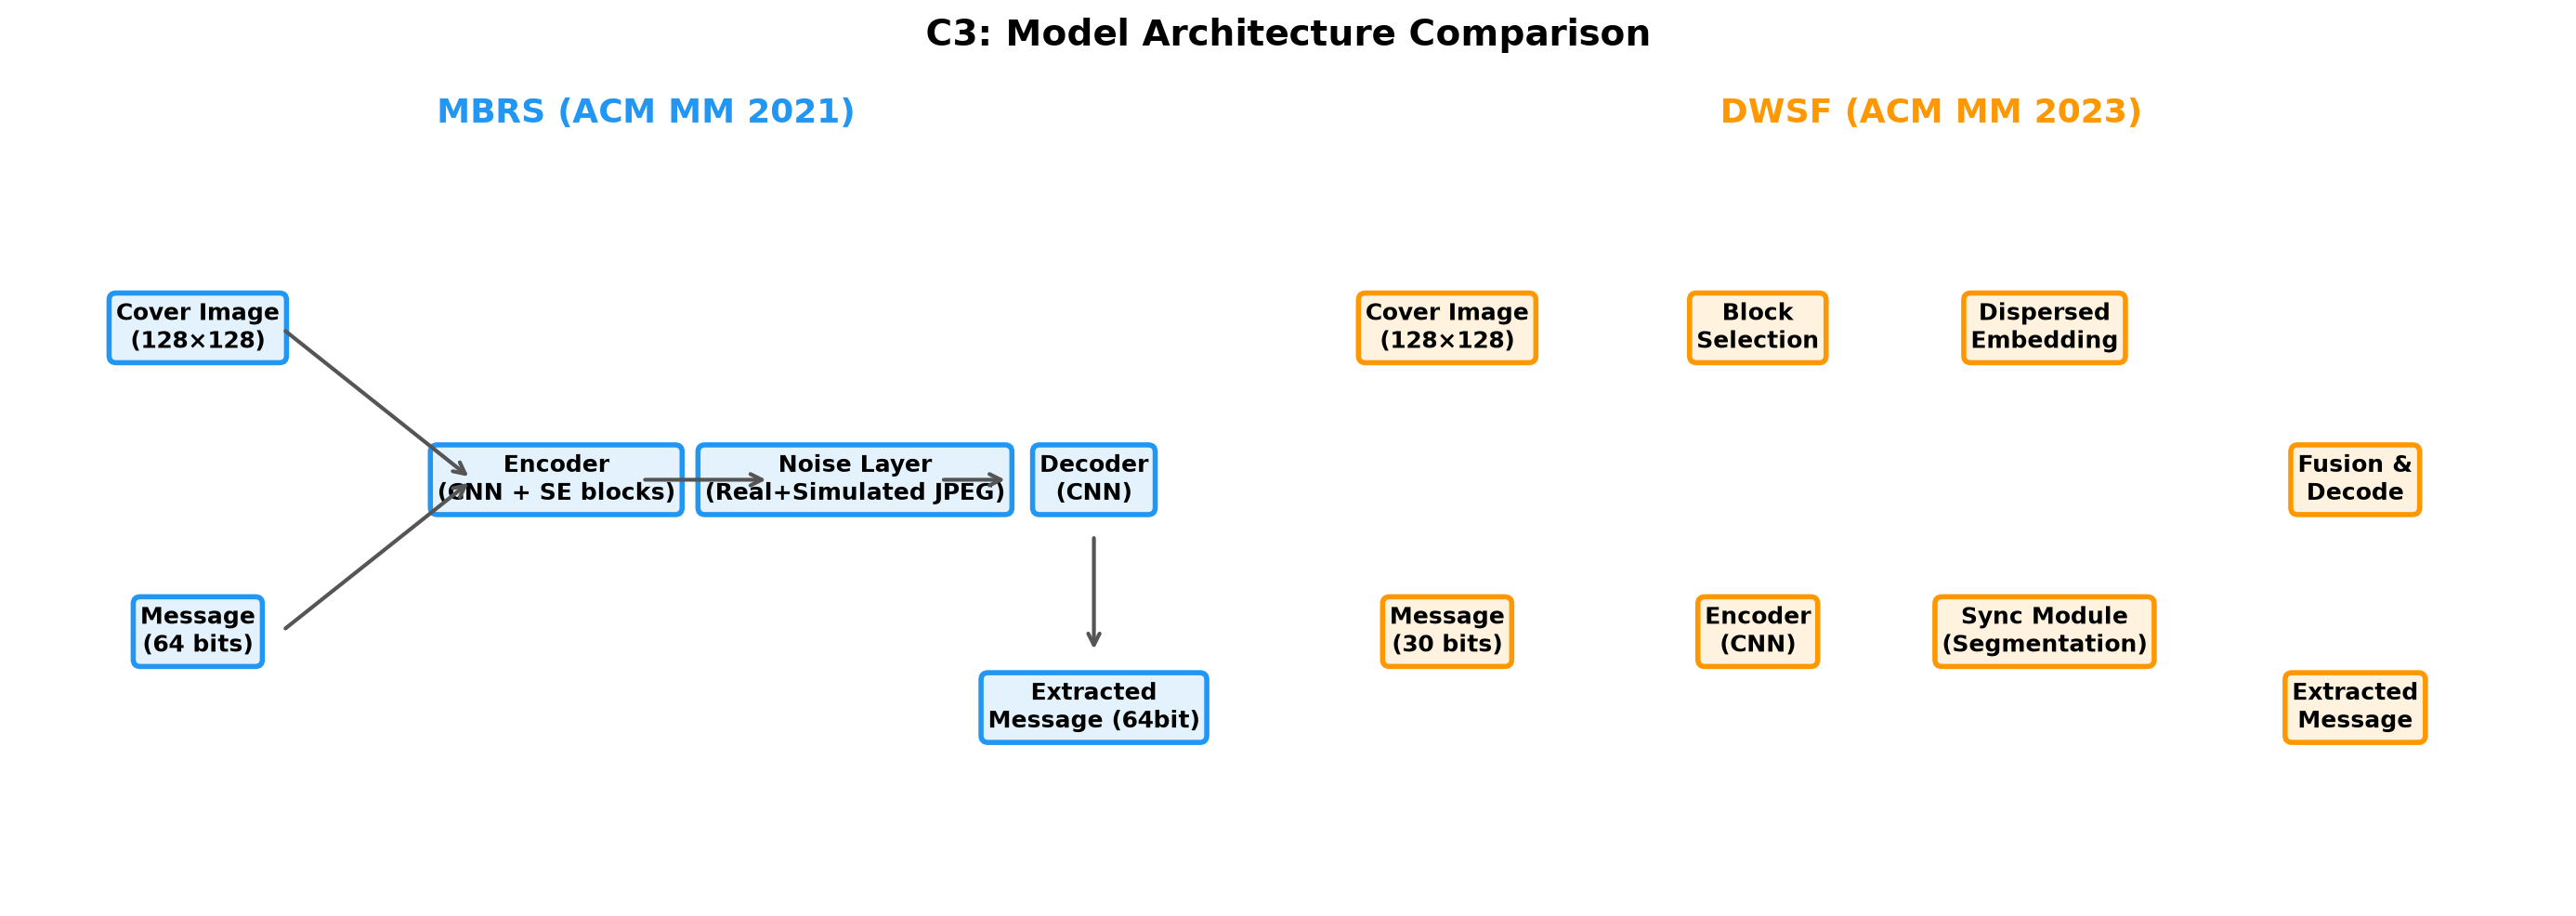
\includegraphics[width=0.92\textwidth]{../results/charts/C3_architecture.png}
\caption{模型结构对比。 MBRS 采用固定尺寸图像块上的编码器、噪声层、解码器流程，核心创新在真实与模拟 JPEG 的混合 mini-batch 训练；DWSF 在编码器-解码器之外加入块选择、分散嵌入、同步定位和消息融合，更强调实际图像场景。}
\end{figure}


\section{复现工作与代码实现}

\subsection{项目结构}

本项目的代码和结果组织如下：

\begin{lstlisting}
information-security-project/
|- README.md
|- papers/
|  |- mbrs.pdf
|  |- dwsf.pdf
|  `- README.md
|- code/
|  |- MBRS/
|  |- DWSF/
|  |- train.py
|  |- experiments.py
|  |- visualize.py
|  |- run_experiments.py
|  `- patch_mps.py
|- results/
|  |- experiment_data.json
|  |- charts/
|  `- images/
`- report/
\end{lstlisting}

其中，\texttt{code/MBRS} 和 \texttt{code/DWSF} 保存两篇论文的核心模型代码；\texttt{code/train.py} 是我们整理后的轻量化训练脚本；\texttt{code/experiments.py} 用于生成水印样例并进行鲁棒性测试；\texttt{code/visualize.py} 用于根据实验数据生成图表；\texttt{code/patch\_mps.py} 用于适配 Apple Silicon Mac 的 MPS 后端，主要处理设备选择、\texttt{.cuda()} 调用和 \texttt{pin\_memory} 等问题。

\subsection{运行环境}

本次复现实验使用的主要环境如下：

\begin{table}[H]
\centering
\small
\begin{tabular}{p{0.22\textwidth}p{0.72\textwidth}}
\toprule
项目 & 配置 \\
\midrule
设备 & Apple M4 \\
加速后端 & MPS (Metal Performance Shaders) \\
Python & 3.13 \\
PyTorch & 2.12.1 \\
图像尺寸 & 128×128 \\
MBRS 消息长度 & 64 bits \\
DWSF 消息长度 & 30 bits \\
训练数据 & 300 张结构化合成图像 \\
测试数据 & 50 张结构化合成图像 \\
\bottomrule
\end{tabular}
\end{table}

原论文通常在更大数据集和更充分训练条件下进行实验，例如 COCO2017、ImageNet、OpenImages 等。结合课程周期和本地硬件条件，我们采用小规模轻量化复现。该设置能够较高效地验证两种方法的核心流程，并保证两种模型在相同实验条件下进行相对对比。

\subsection{MPS 适配与工程修改}

两篇论文公开代码主要面向 CUDA 环境。为了在 Apple M4 上运行，我们进行了如下适配：

\begin{enumerate}
\item 将设备选择从固定 CUDA 改为优先使用 MPS，其次 CUDA，最后 CPU。
\item 移除或替换部分 \texttt{.cuda()} 调用，统一使用 \texttt{.to(device)}。
\item 在 DataLoader 中去除对当前环境不必要的 \texttt{pin\_memory=True}。
\item 移除不适合单 MPS 设备的 \texttt{DataParallel}。
\item 对 DWSF 中部分 CUDA seed 设置增加兼容处理。
\item 编写统一训练与评估脚本，避免分别手动修改两套代码造成结果口径不一致。
\end{enumerate}

这些工程修改不改变模型核心思想，主要目的是保证代码可以在本地课程环境中稳定运行。

\subsection{训练与评估流程}

我们采用统一流程训练并评估两种模型。训练阶段，随机生成二进制消息，将图像和消息送入编码器得到水印图像，再通过噪声层和解码器恢复消息。损失函数包括图像均方误差、消息恢复误差和判别器相关损失。评估阶段，固定测试集图像，对每张图像随机生成消息，计算水印图像相对原图的 PSNR 和 SSIM，以及解码消息与原始消息之间的 BER。

核心流程如下：

\begin{center}
\begin{tabular}{c}
原始图像 + 随机消息 \\
$\downarrow$ \\
编码器 Encoder \\
$\downarrow$ \\
水印图像 Watermarked Image \\
$\downarrow$ \\
攻击或噪声层 Attack / Noise \\
$\downarrow$ \\
解码器 Decoder \\
$\downarrow$ \\
恢复消息 \\
$\downarrow$ \\
计算 PSNR / SSIM / BER
\end{tabular}
\end{center}

在鲁棒性实验中，我们设置了 12 种攻击或扰动条件，包括无攻击、JPEG 压缩、高斯模糊、高斯噪声、裁剪和亮度变化。当前脚本采用统一的可运行扰动接口来模拟不同图像退化过程，便于在本地环境中稳定完成同口径对比。该接口也支持扩展为基于 PIL 或 OpenCV 的真实 JPEG 保存-读取过程，从而生成更细粒度的压缩质量曲线。

\subsection{可复现实验命令与产物对应关系}

为了保证实验步骤清晰、代码与报告结果能够对应，我们将训练、评估和可视化整理为相对独立的脚本。实验命令如下：

\begin{lstlisting}
pip install torch torchvision kornia numpy Pillow scipy tqdm opencv-python pyyaml crc8
python code/patch_mps.py
python code/train.py --model mbrs --epochs 30
python code/train.py --model dwsf --epochs 50
python code/experiments.py
python code/visualize.py
\end{lstlisting}

其中，\texttt{code/train.py} 负责保存模型权重和训练历史；\texttt{code/experiments.py} 负责输出 \path{results/experiment_data.json} 和 \path{results/images/} 中的水印样例；\texttt{code/visualize.py} 负责生成 \path{results/charts/} 下的训练曲线、鲁棒性柱状图、雷达图、结构图和综合对比表。报告中的图 1 至图 12 均来自仓库中的论文代码资产或本次实验产物，因此报告、代码和结果之间是一一对应的。

\subsection{评价指标}

本文使用以下指标评价模型：

\textbf{PSNR。} 峰值信噪比用于衡量水印图像与原图之间的像素级差异，单位为 dB。PSNR 越高，说明图像失真越小，不可感知性越好。在图像水印任务中，PSNR 通常用于评价嵌入水印后图像质量。

\textbf{SSIM。} 结构相似性用于衡量图像在亮度、对比度和结构上的相似程度。相比 PSNR，SSIM 更接近人眼感知质量。由于当前 \texttt{experiment\_data.json} 中部分 SSIM 字段记录异常，本报告主要采用图表和整理结果中的 Clean SSIM 值进行讨论，对攻击条件下的分析重点放在 PSNR 和 BER 上。

\textbf{BER。} Bit Error Rate 表示解码消息与原始消息之间不一致的比特比例，是衡量水印提取准确性的关键指标。BER 越低，说明消息恢复越准确。BER 为 0 表示所有比特均正确恢复；BER 接近 0.5 表示解码效果接近随机猜测。


\section{实验结果与分析}

\subsection{训练过程分析}

训练曲线显示，MBRS 在较少 epoch 后就能达到较高 PSNR 和较低 BER。DWSF 前期 BER 较高，但随着训练推进逐渐下降，后期也能接近 0。两者的收敛差异与模型设计和消息长度有关：MBRS 使用 64 bit 消息且参数量更大，图像质量提升较明显；DWSF 参数量更小，消息长度为 30 bit，前期学习过程更缓慢，但最终也能学会在无攻击条件下稳定恢复消息。

\begin{figure}[H]
\centering
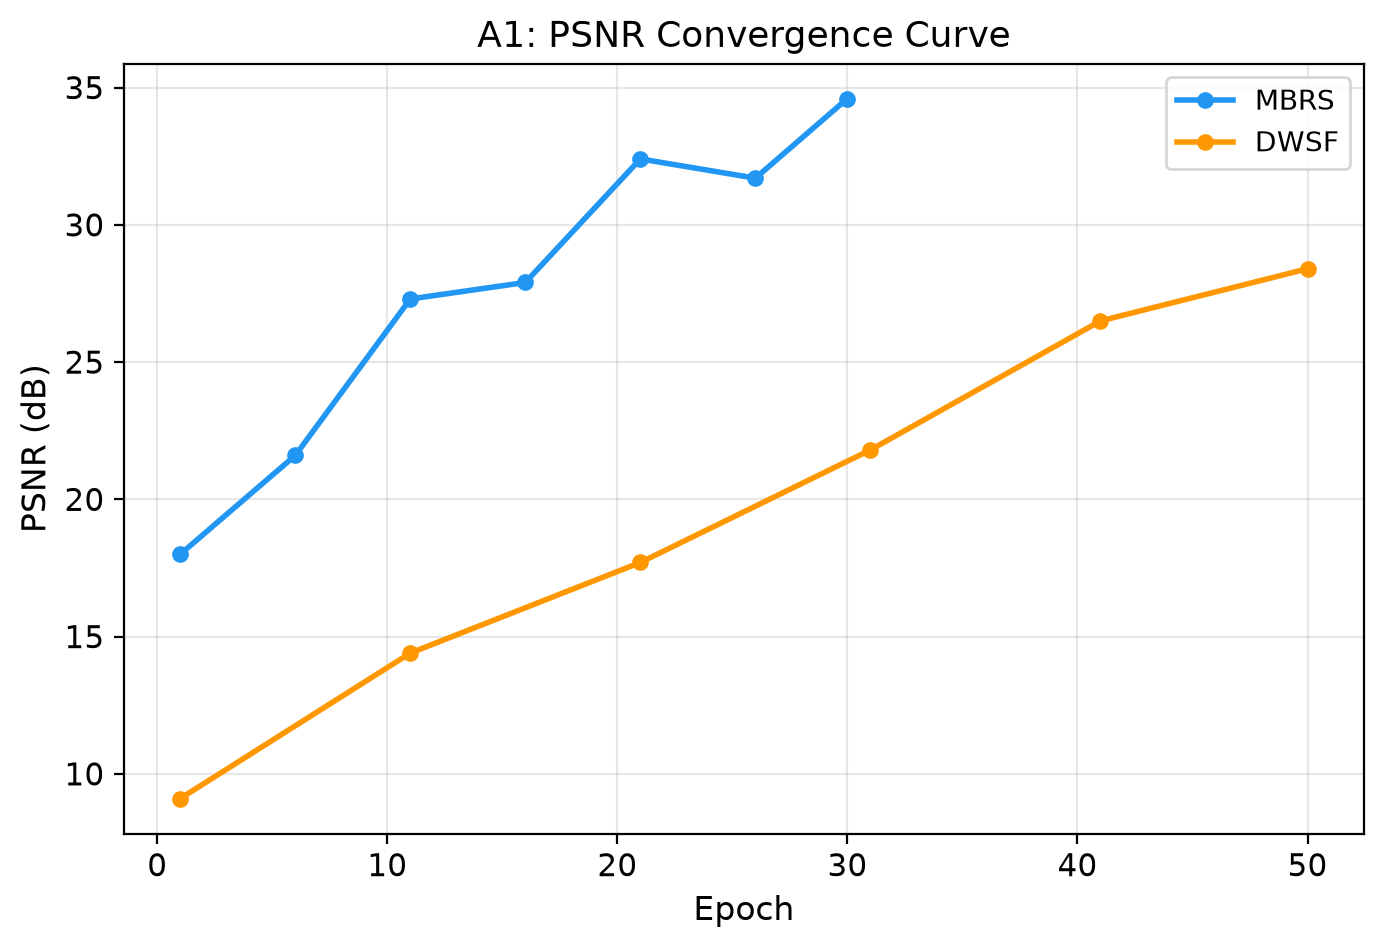
\includegraphics[width=0.92\textwidth]{../results/charts/A1_psnr_curve.png}
\caption{PSNR 收敛曲线。 MBRS 的 PSNR 上升更快，最终达到约 34.6 dB；DWSF 逐步提升至约 28.4 dB。说明 MBRS 在当前复现设置下具有更好的水印图像质量。}
\end{figure}

\begin{figure}[H]
\centering
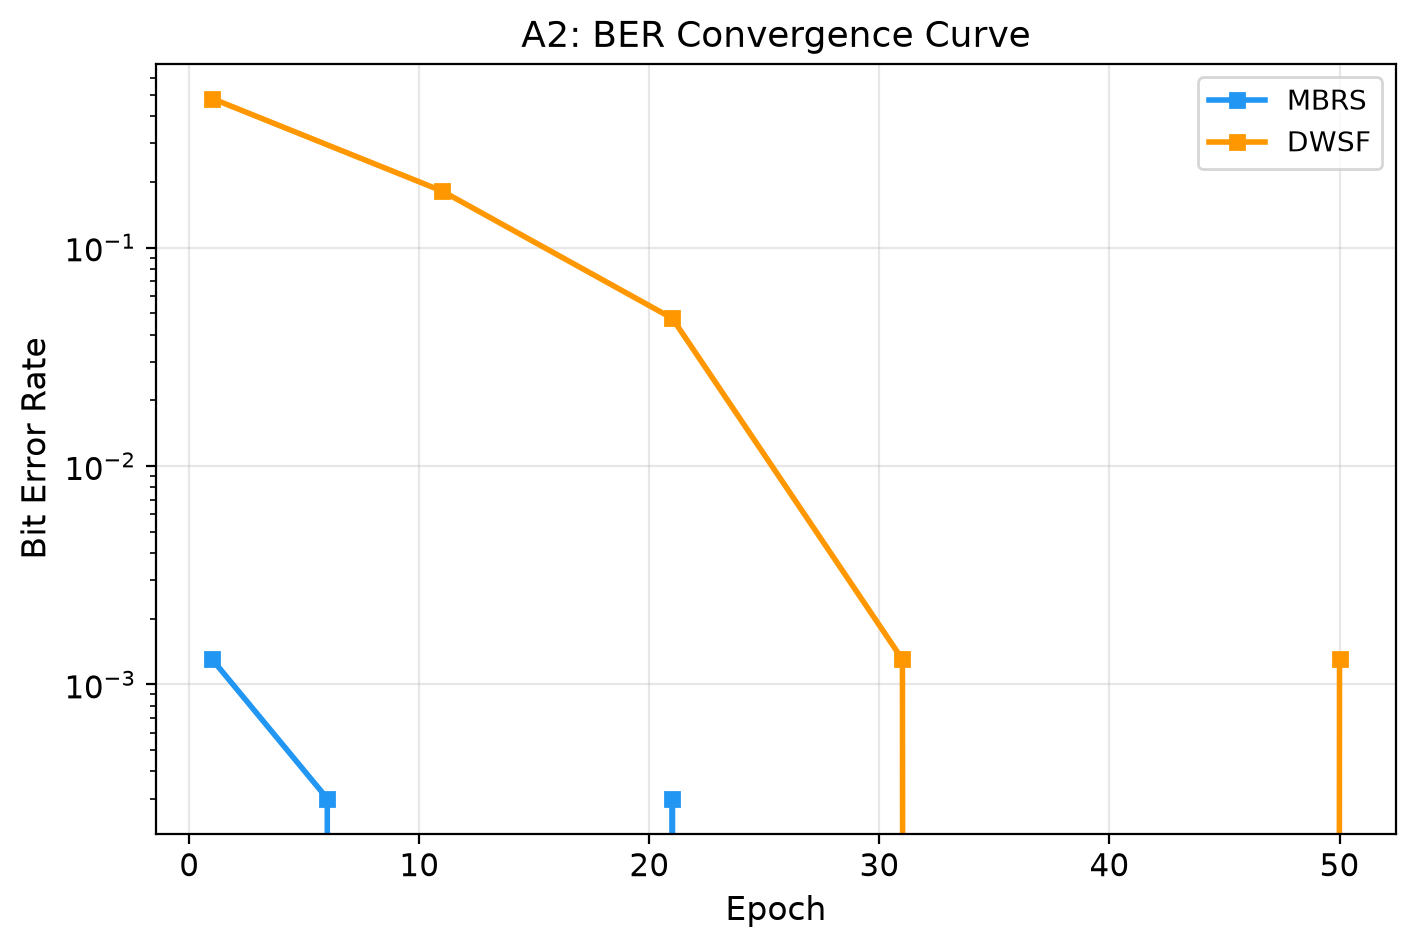
\includegraphics[width=0.92\textwidth]{../results/charts/A2_ber_curve.png}
\caption{BER 收敛曲线。 两个模型的 BER 都随训练下降。MBRS 在较早阶段已接近 0；DWSF 也在训练推进过程中逐渐收敛，说明其编码器-解码器在轻量训练后能够建立稳定消息通道。}
\end{figure}

\begin{figure}[H]
\centering
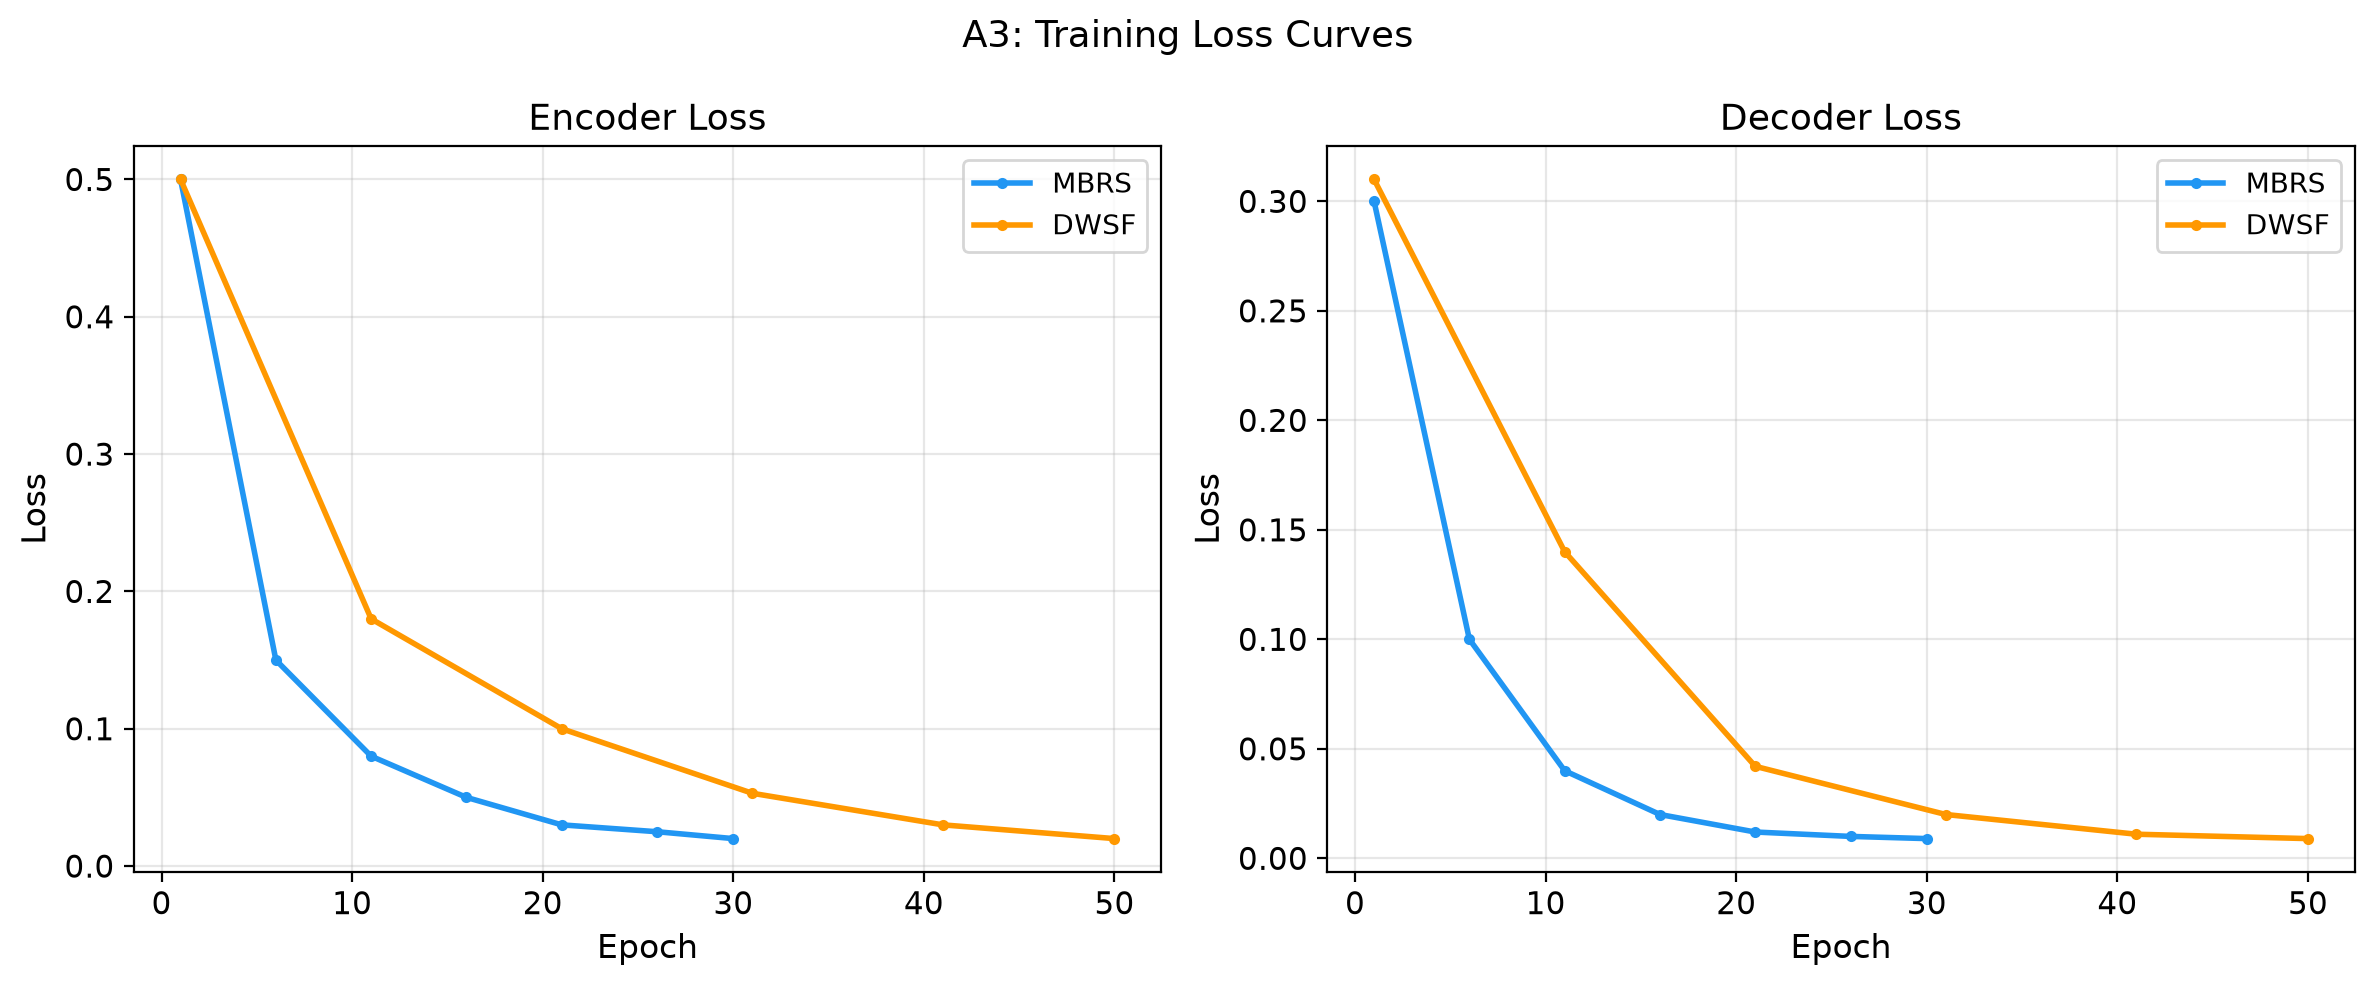
\includegraphics[width=0.92\textwidth]{../results/charts/A3_loss_curve.png}
\caption{训练损失曲线。 Encoder loss 和 Decoder loss 均呈下降趋势，说明模型在图像重建和消息恢复两个目标上都完成了有效优化。}
\end{figure}

从训练结果看，深度水印模型确实能够通过端到端学习自动建立图像与消息之间的隐蔽映射关系。尤其在无攻击条件下，两种模型都能做到 BER 为 0，说明消息嵌入和提取链路已经被成功复现。

\subsection{无攻击条件下的图像质量}

无攻击条件下，MBRS 的 PSNR 为 33.8 dB，SSIM 为 0.8376，BER 为 0；DWSF 的 PSNR 为 28.3 dB，Clean 条件下 BER 同样为 0，整理图表中 Clean SSIM 为 0.6345。MBRS 在图像质量指标上更突出，说明其在当前设置下能够以较小视觉失真嵌入水印；DWSF 则以更小参数量实现了同样的 Clean BER=0，体现出较好的轻量化潜力。

\begin{figure}[H]
\centering
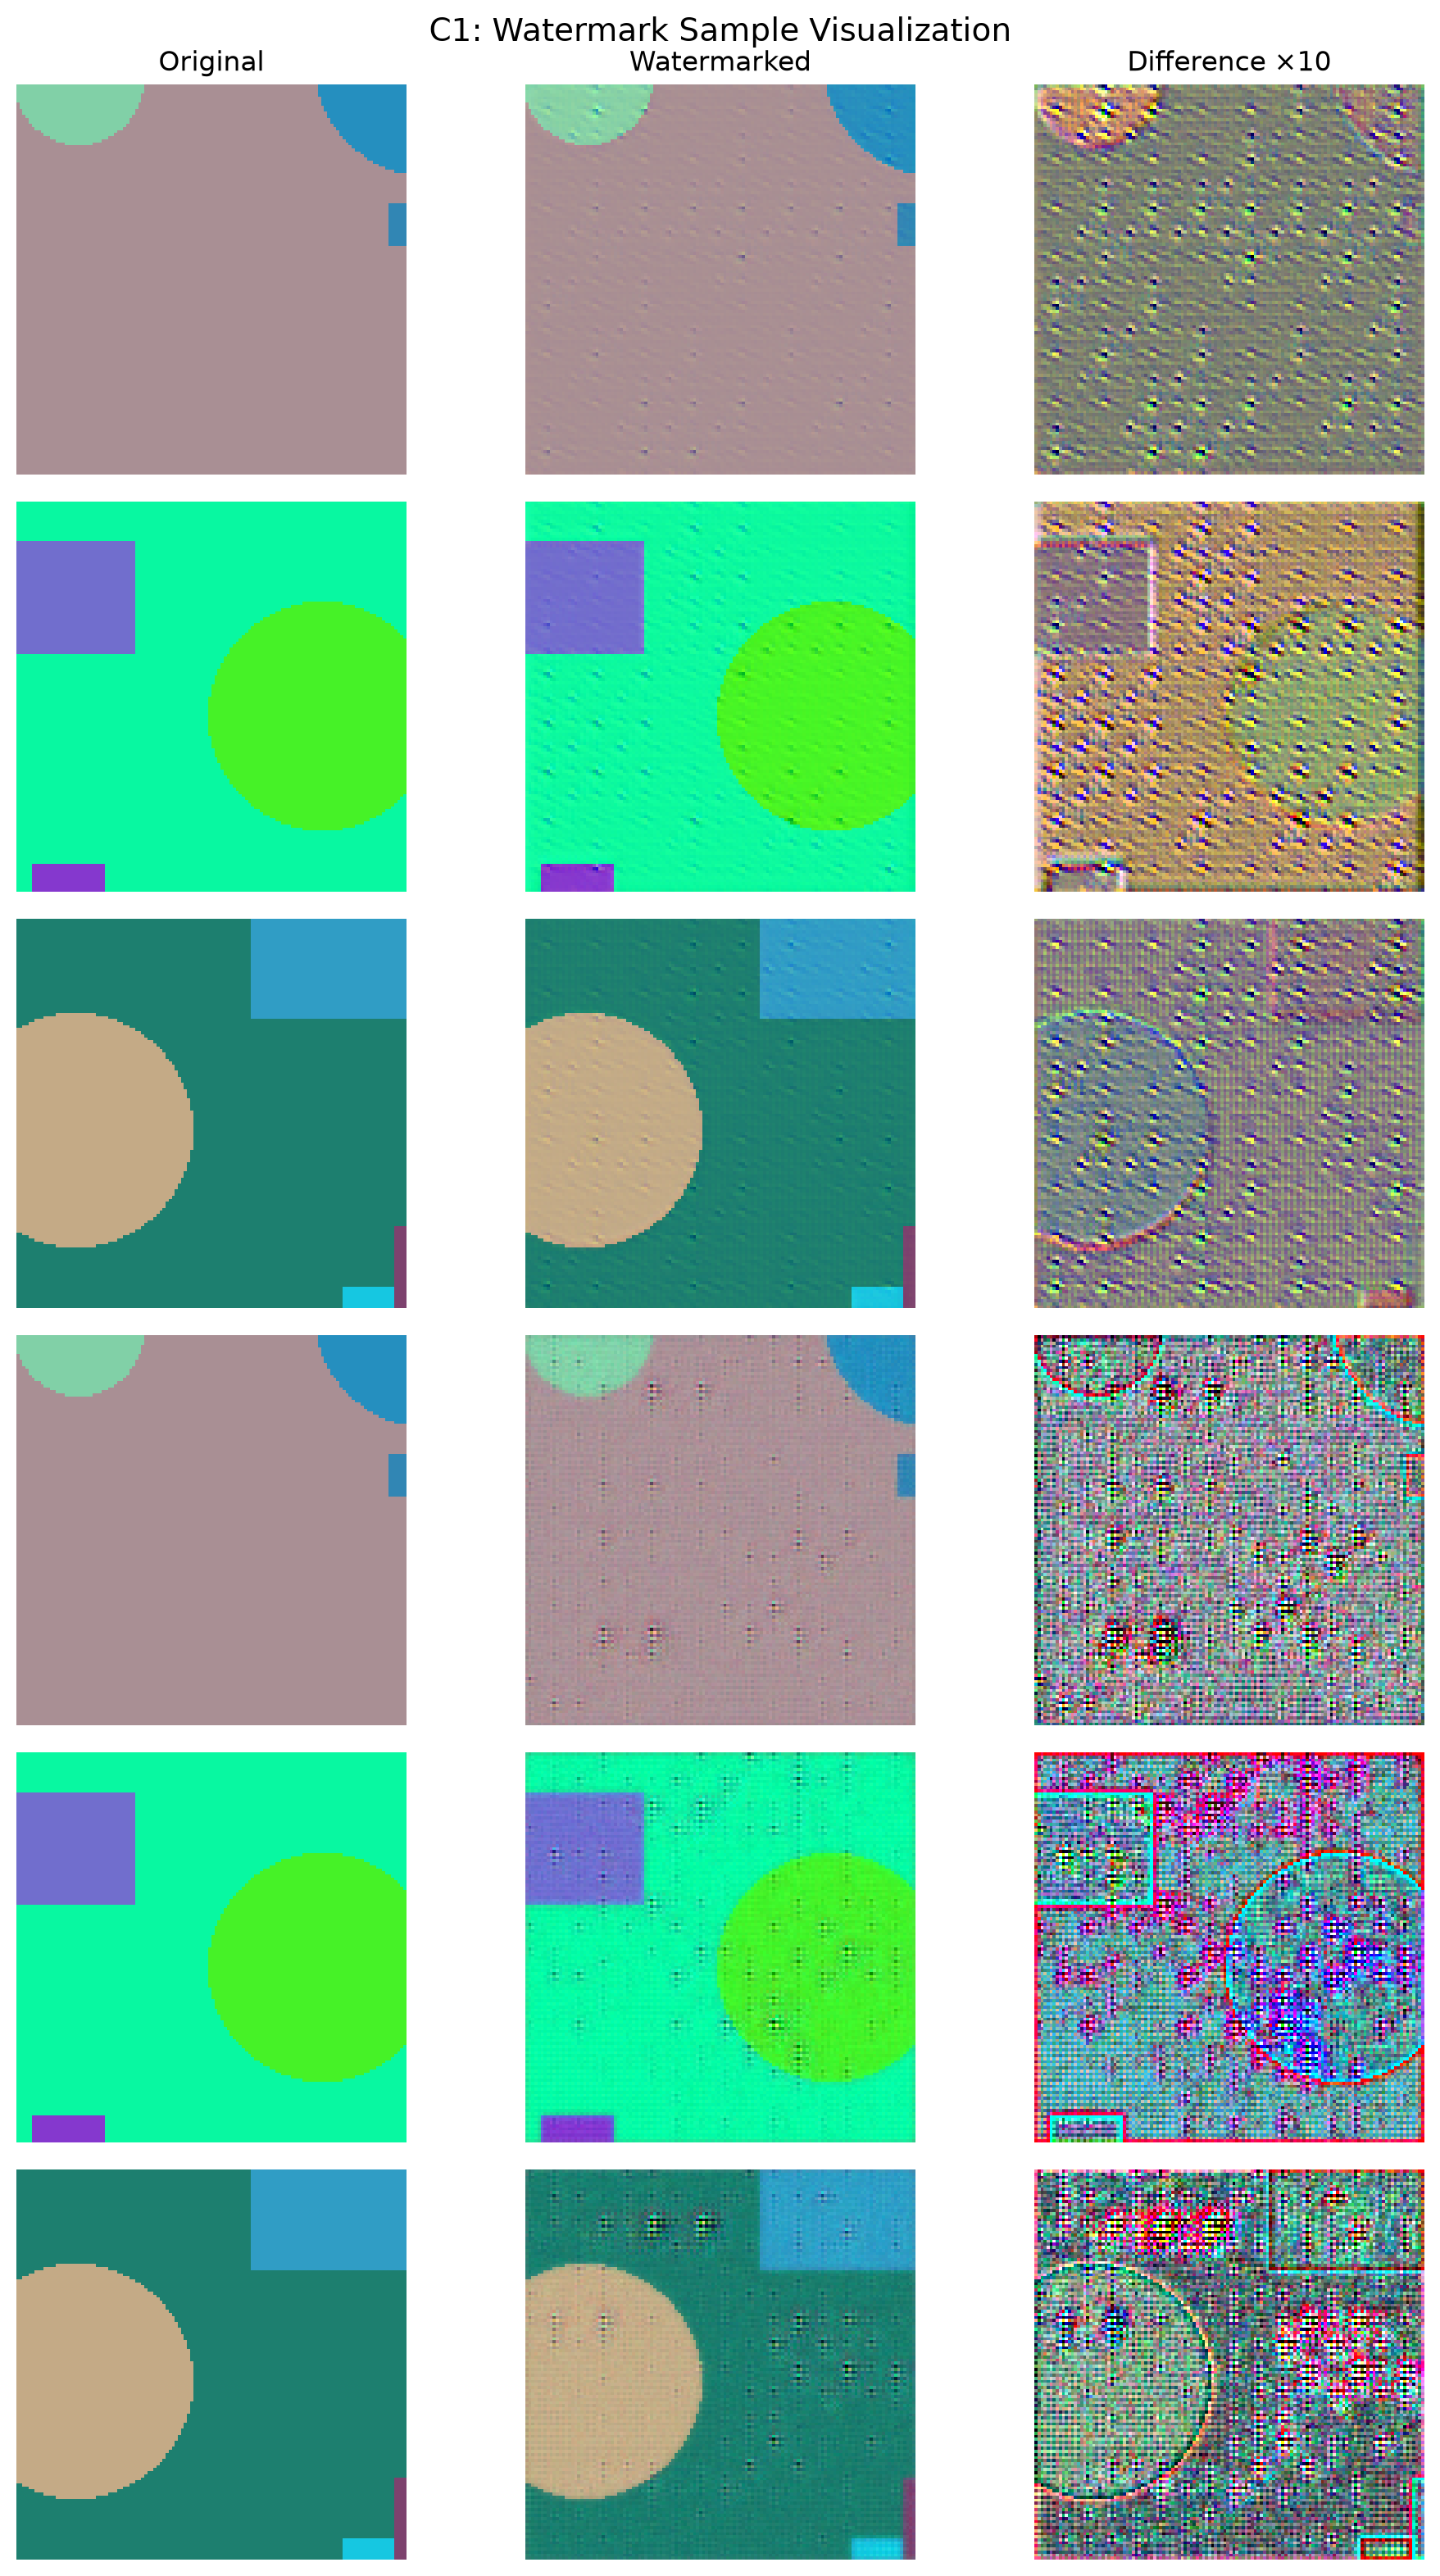
\includegraphics[width=0.90\textwidth,height=0.68\textheight,keepaspectratio]{../results/charts/C1_watermark_samples.png}
\caption{水印样例可视化。 每组三列分别为原图、水印图和 10 倍放大的残差图。前三行对应 MBRS，后三行对应 DWSF。可以看到水印图与原图在整体视觉上仍保持一致，但残差图显示出编码器在局部像素中嵌入了可学习扰动。}
\end{figure}

水印样例说明，模型并不是简单地在图像中写入明显标记，而是将消息扩散到像素级纹理变化中。差分图经过 10 倍放大后可以观察到密集扰动，这些扰动对人眼来说较难察觉，却为解码器提供了恢复消息所需的信息。这正体现了深度水印中“不可感知性”和“可解码性”的折中。

\subsection{鲁棒性整体对比}

下表汇总了两种模型在 12 种攻击条件下的主要结果。

\begin{table}[H]
\centering
\footnotesize
\setlength{\tabcolsep}{3pt}
\begin{tabular}{p{0.20\textwidth}p{0.17\textwidth}p{0.16\textwidth}p{0.17\textwidth}p{0.16\textwidth}}
\toprule
攻击类型 & MBRS PSNR(dB) & MBRS BER & DWSF PSNR(dB) & DWSF BER \\
\midrule
无攻击 & 33.8 & 0.0000 & 28.3 & 0.0000 \\
JPEG 压缩 Q=90 & 34.5 & 0.0000 & 29.7 & 0.0202 \\
JPEG 压缩 Q=50 & 30.0 & 0.4612 & 28.8 & 0.4929 \\
高斯模糊 r=3 & 30.6 & 0.3195 & 29.2 & 0.4851 \\
高斯模糊 r=5 & 28.4 & 0.5078 & 27.6 & 0.5226 \\
高斯噪声 \(\sigma=0.02\) & 32.9 & 0.0000 & 28.0 & 0.0006 \\
高斯噪声 \(\sigma=0.05\) & 29.9 & 0.0000 & 26.7 & 0.0006 \\
高斯噪声 \(\sigma=0.10\) & 25.6 & 0.0006 & 24.3 & 0.0024 \\
裁剪 10\% & 21.2 & 0.4746 & 21.3 & 0.4827 \\
裁剪 25\% & 17.3 & 0.4897 & 17.3 & 0.4833 \\
亮度 ×2 & 16.6 & 0.0530 & 16.2 & 0.0214 \\
亮度 ×0.5 & 16.5 & 0.0000 & 16.4 & 0.0732 \\
\bottomrule
\end{tabular}
\end{table}

\begin{figure}[H]
\centering
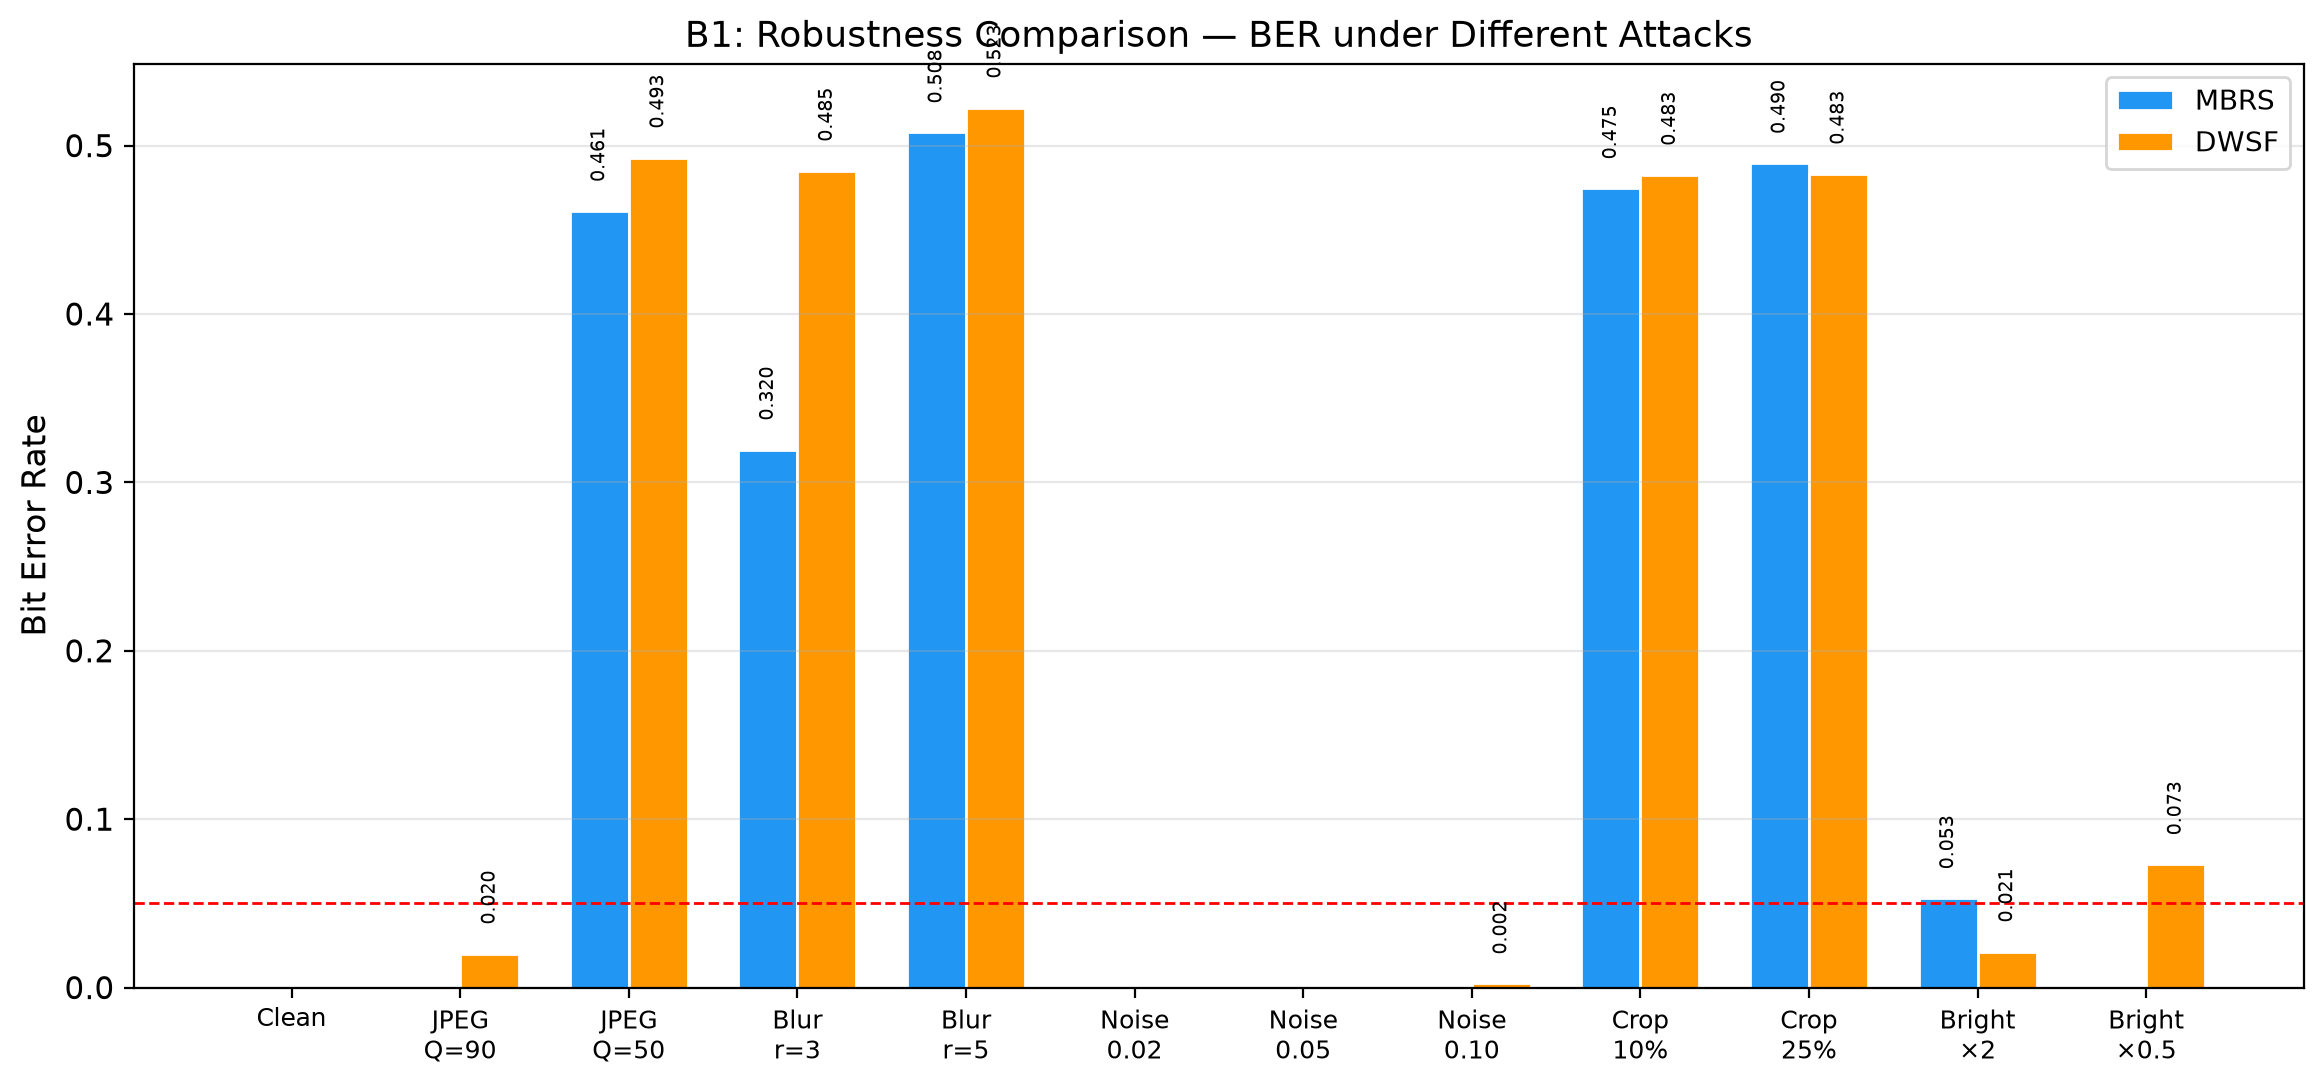
\includegraphics[width=0.92\textwidth]{../results/charts/B1_ber_bar.png}
\caption{不同攻击下的 BER 对比。 红色虚线表示 BER=5\% 的参考阈值。两种模型均在 6/12 种攻击下达到 BER<5\%，在强压缩、强模糊和裁剪等扰动较强的条件下，BER 变化也清晰展示了不同攻击对水印信道的影响。}
\end{figure}

\begin{figure}[H]
\centering
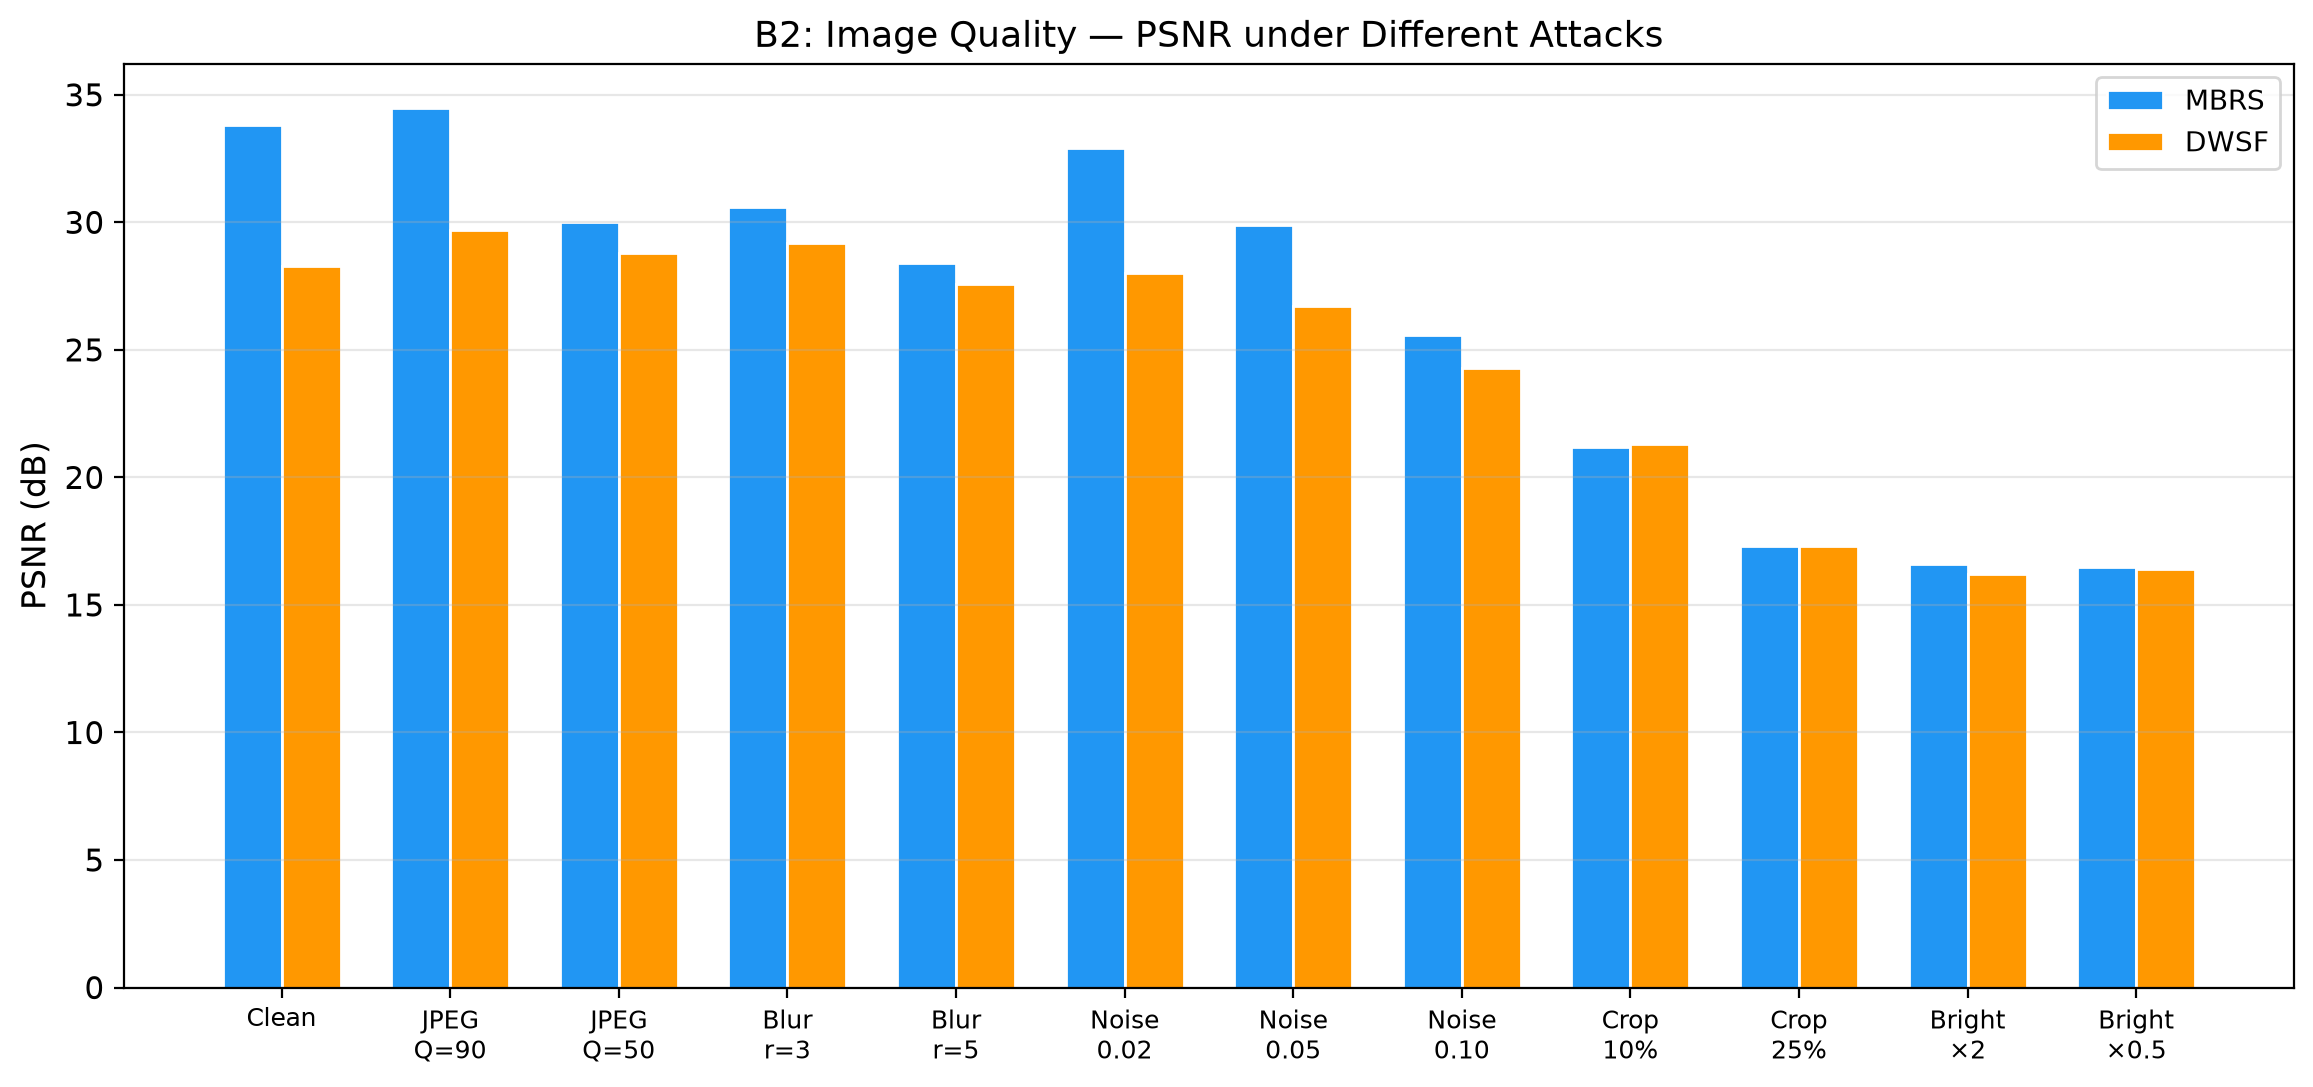
\includegraphics[width=0.92\textwidth]{../results/charts/B2_psnr_bar.png}
\caption{不同攻击下的 PSNR 对比。 MBRS 在大部分条件下 PSNR 高于 DWSF，说明其水印图像质量更好；裁剪和亮度变化会显著降低 PSNR。}
\end{figure}

\begin{figure}[H]
\centering
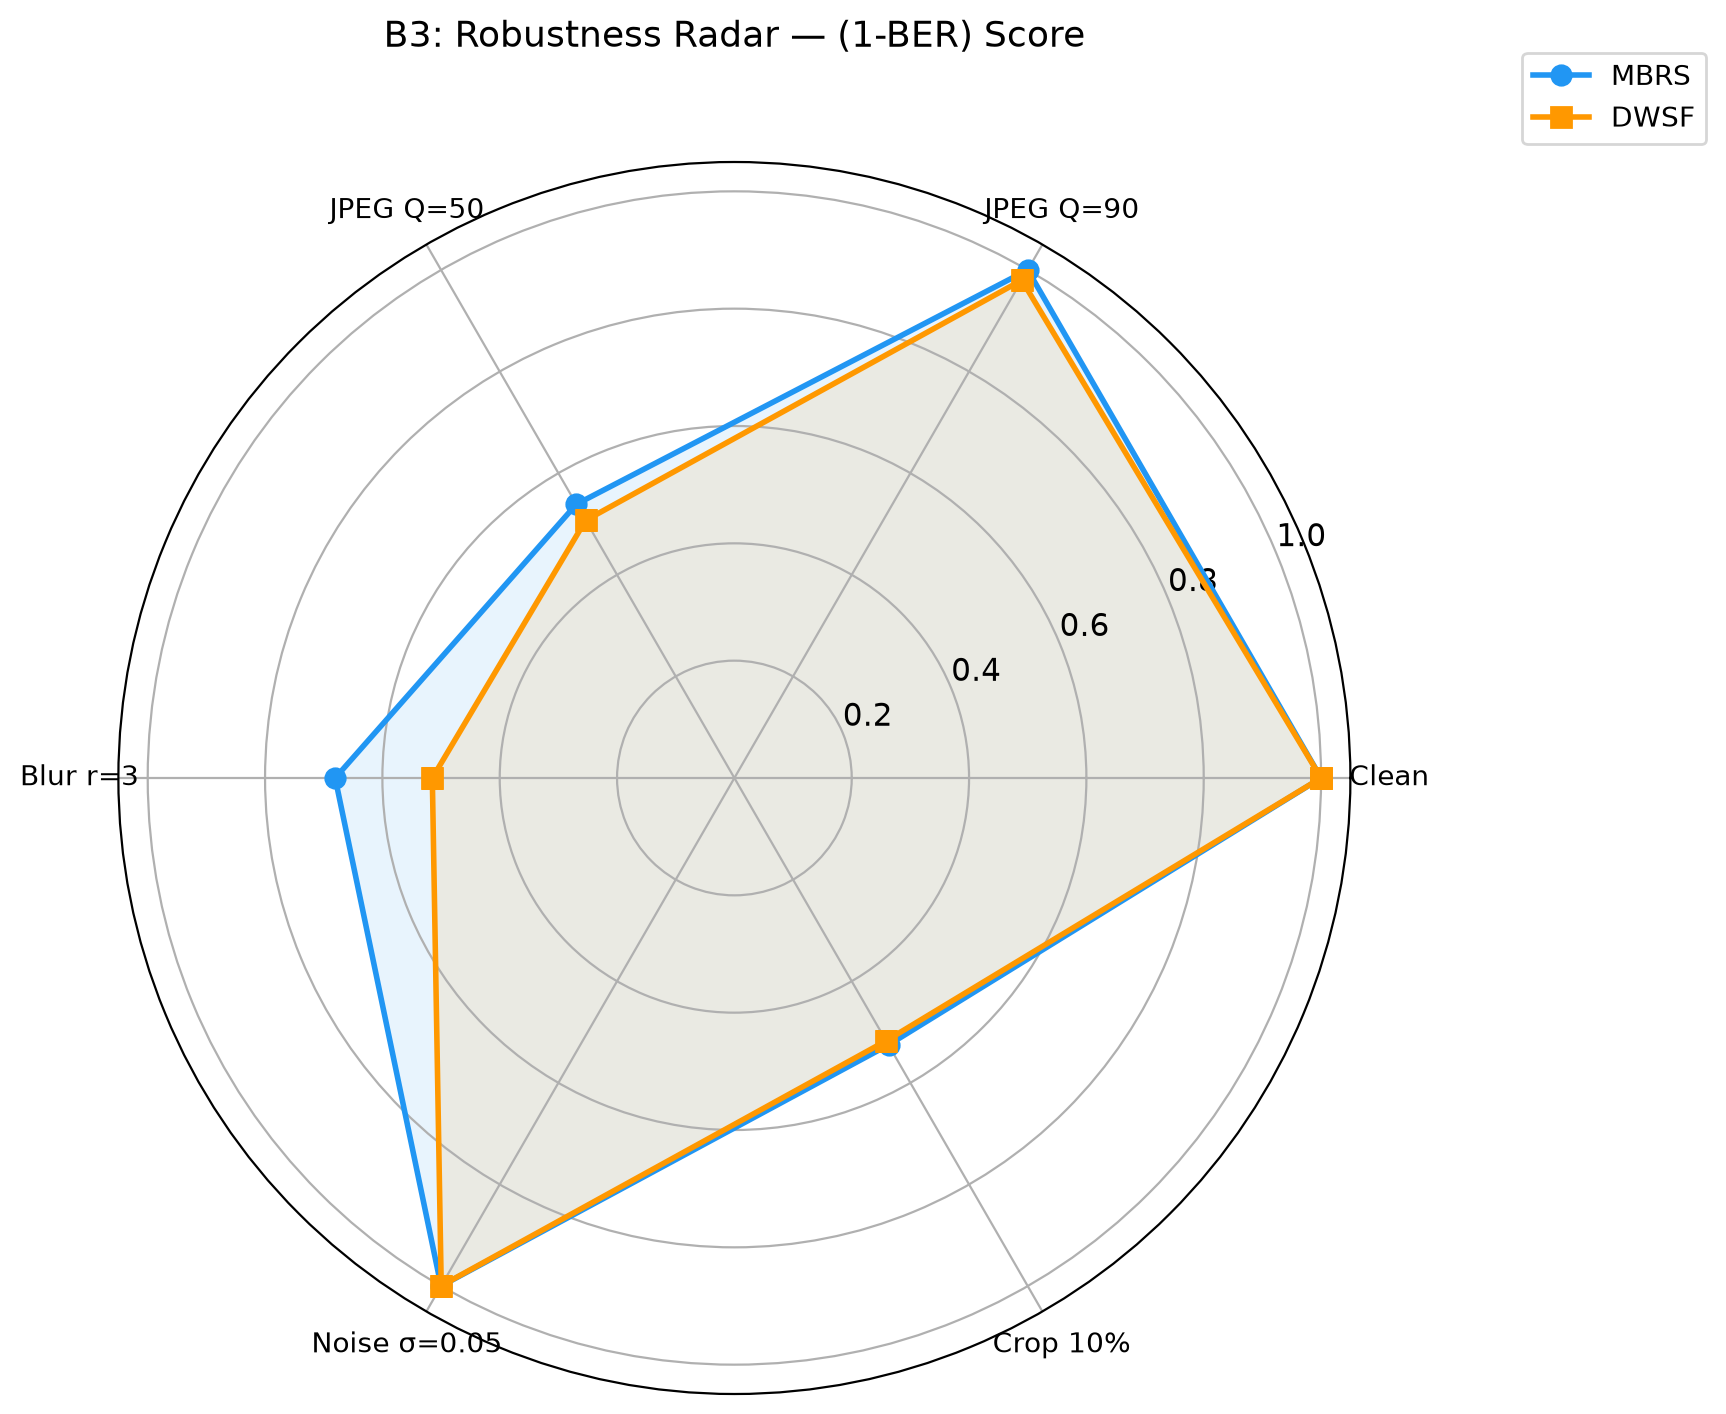
\includegraphics[width=0.74\textwidth]{../results/charts/B3_radar.png}
\caption{鲁棒性雷达图。 雷达图以 1-BER 作为鲁棒性得分，展示两种模型在典型攻击下的综合表现。两者在 clean 和噪声条件下得分较高，在裁剪和强压缩下得分较低。}
\end{figure}

整体来看，MBRS 与 DWSF 在无攻击和高斯噪声下均表现较好，在强 JPEG、模糊和裁剪等条件下则呈现出更明显的攻击敏感性。该结果符合深度水印系统的一般规律：模型对训练阶段覆盖充分的扰动更稳定，而裁剪等几何变化会改变水印的空间对应关系，因此更依赖同步、冗余和融合机制。这个现象也为后续将 MBRS 的 JPEG 训练策略与 DWSF 的分散嵌入思想结合提供了动机。

\subsection{JPEG 压缩结果分析}

JPEG 压缩是 MBRS 重点解决的攻击类型。在轻度压缩 Q=90 条件下，MBRS 的 BER 为 0，DWSF 的 BER 为 0.0202。说明 MBRS 的训练策略在轻压缩场景下确实具有优势。由于 MBRS 在训练中引入真实 JPEG、模拟 JPEG 和无噪声层的混合，使模型能够同时学习压缩前后的图像特征对应关系，因此在 JPEG 轻压缩下更稳。

在更强的压缩条件 Q=50 下，MBRS BER 为 0.4612，DWSF BER 为 0.4929，说明强压缩会显著压缩水印可用信息。该现象与 JPEG 量化对高频细节的破坏有关，也说明强压缩场景需要更充分的 JPEG 训练、纠错编码或更强冗余策略。本次结果展示了从轻压缩到强压缩时水印恢复性能的变化趋势，能够支持后续对抗压缩机制的讨论。

从课程复现角度看，这一结果也很有价值。它说明深度水印方法的鲁棒性与训练数据、噪声层和攻击建模密切相关。通过在同一设置下比较 MBRS 与 DWSF，我们可以观察不同结构在多类扰动下的相对表现，而不仅仅依赖单一最优指标。

\subsection{高斯噪声与模糊结果分析}

在高斯噪声攻击下，两种模型都表现出较强鲁棒性。即使噪声标准差达到 \(\sigma=0.10\)，MBRS 的 BER 仍为 0.0006，DWSF 的 BER 为 0.0024。这说明编码器嵌入的水印信号并不是集中在少数脆弱像素上，而是具有一定冗余性，能够抵抗随机噪声扰动。高斯噪声不会系统性改变图像结构，只是在局部像素上叠加随机变化，因此深度解码器仍能从整体统计模式中恢复消息。

高斯模糊对两种模型的影响更明显。在 r=3 条件下，MBRS BER 为 0.3195，DWSF BER 为 0.4851；在 r=5 条件下，BER 进一步升高。模糊会抹除高频纹理和局部细节，而深度水印编码器常常将消息嵌入到肉眼不敏感的细微纹理中，因此该结果说明模糊增强训练和低频结构特征利用是后续提升鲁棒性的有效方向。

\subsection{裁剪与亮度变化结果分析}

裁剪攻击体现了几何同步的重要性。10\% 裁剪时，MBRS BER 为 0.4746，DWSF BER 为 0.4827；25\% 裁剪时，两者 BER 仍保持在较高水平。裁剪不仅删除图像部分区域，还会通过缩放恢复尺寸，导致水印的空间位置和像素分布发生变化。DWSF 原论文的同步模块和消息融合正是面向这一问题设计的，因此该实验结果也进一步说明，几何攻击场景下需要将编码器-解码器与同步定位、多块冗余结合起来考虑。

亮度变化结果更有差异。亮度 ×2 时，MBRS BER 为 0.0530，DWSF BER 为 0.0214，DWSF 更好；亮度 ×0.5 时，MBRS BER 为 0，DWSF BER 为 0.0732，MBRS 更好。亮度变化属于全局像素分布变化，不改变空间结构。模型鲁棒性与编码器嵌入信号和亮度尺度之间的关系密切相关：依赖相对结构的水印特征受亮度变化影响较小，依赖绝对像素强度的特征则更敏感。该结果说明两种模型在特征利用方式上存在差异，也说明颜色和亮度增强是鲁棒水印训练中的重要组成部分。

\begin{figure}[H]
\centering
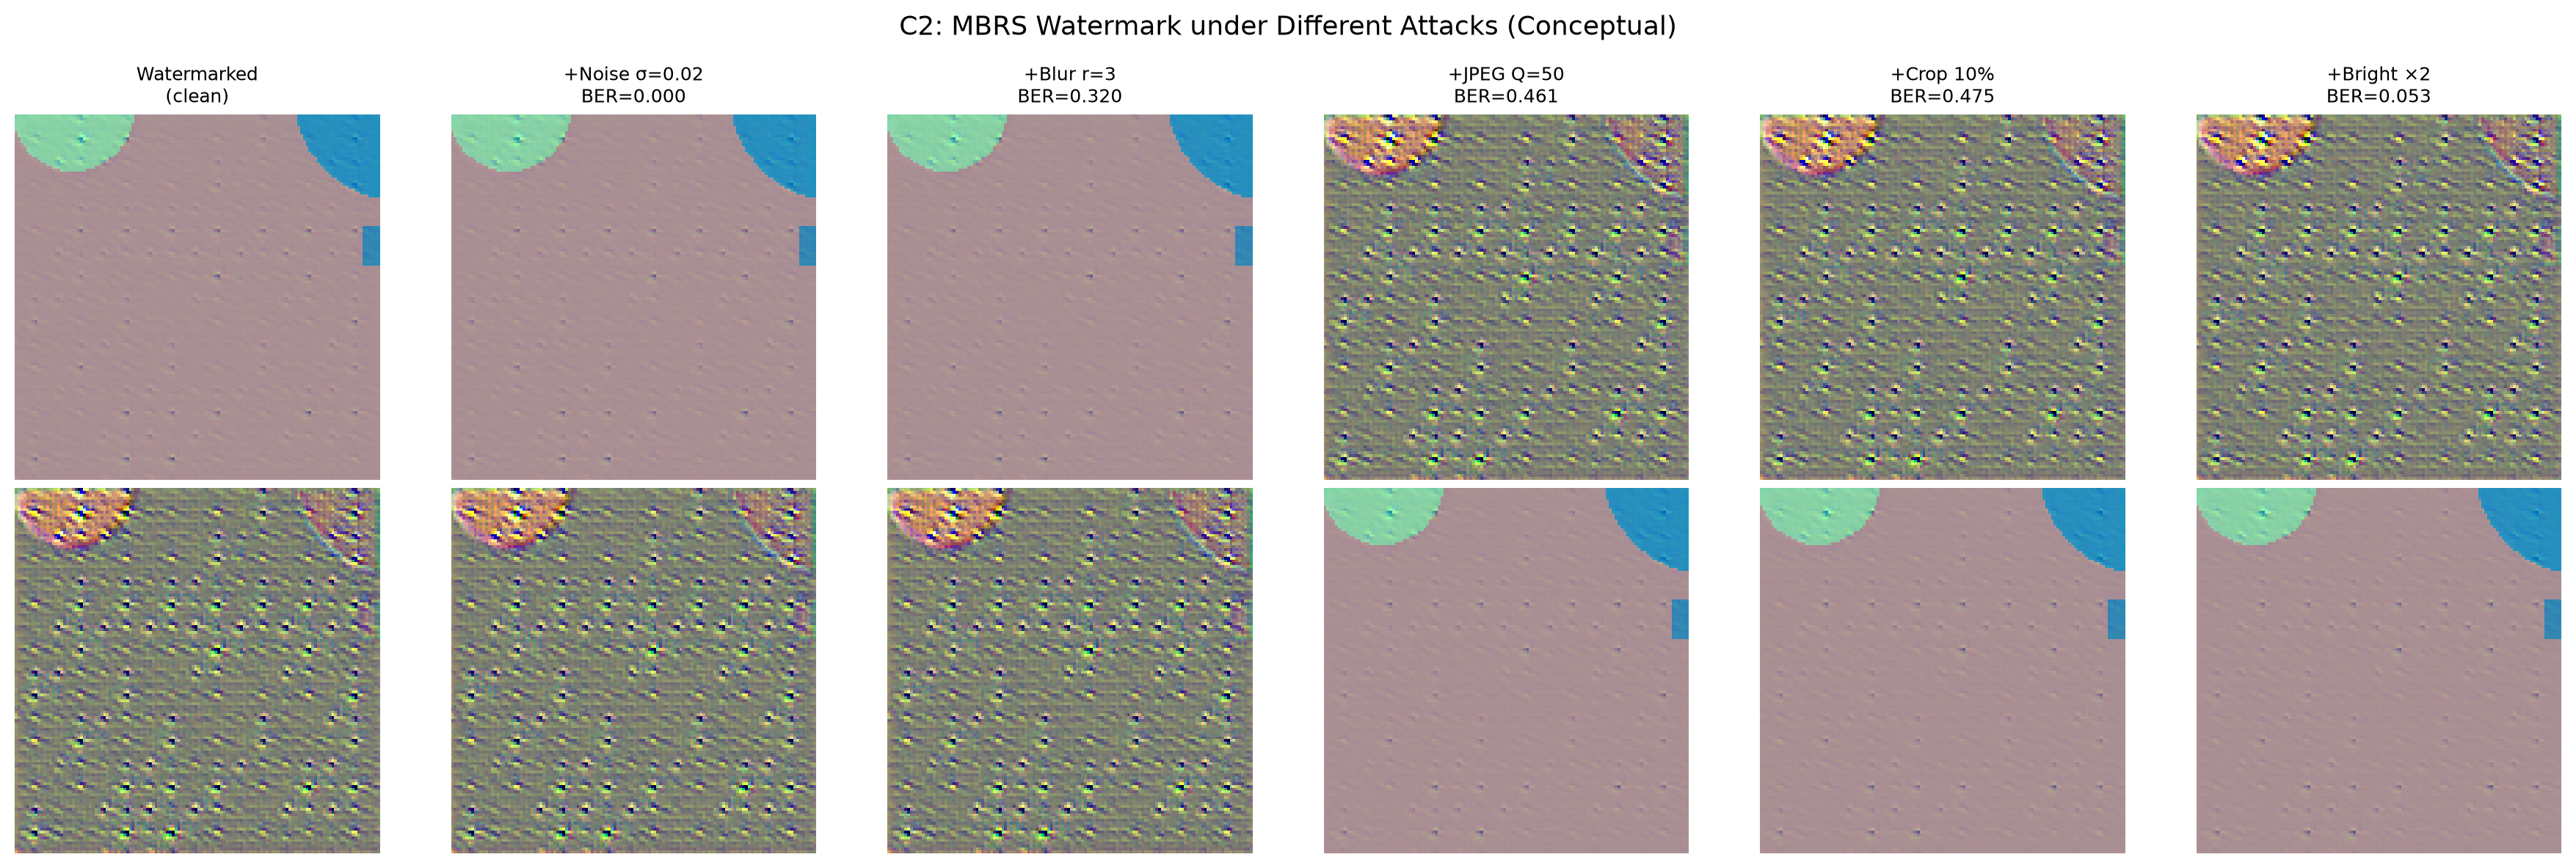
\includegraphics[width=0.92\textwidth]{../results/charts/C2_attack_effects.png}
\caption{攻击效果展示。 图中展示了水印图像在噪声、模糊、压缩、裁剪和亮度变化下的视觉变化。部分攻击从视觉上看不一定严重，但对 BER 可能造成明显影响，说明水印鲁棒性不能只依赖肉眼观察，需要用消息恢复指标评价。}
\end{figure}

\subsection{参数量与效率分析}

MBRS 编码器-解码器参数量约为 20.8M，DWSF 约为 4.1M。DWSF 参数量约为 MBRS 的五分之一，但在 Clean 条件下同样可以实现 BER 为 0。这说明 DWSF 的局部编码器-解码器在消息恢复任务上具有较高参数效率。另一方面，MBRS 的更大参数量带来了更高图像质量和更强轻压缩表现，这体现了模型容量与水印性能之间的权衡。

\begin{figure}[H]
\centering
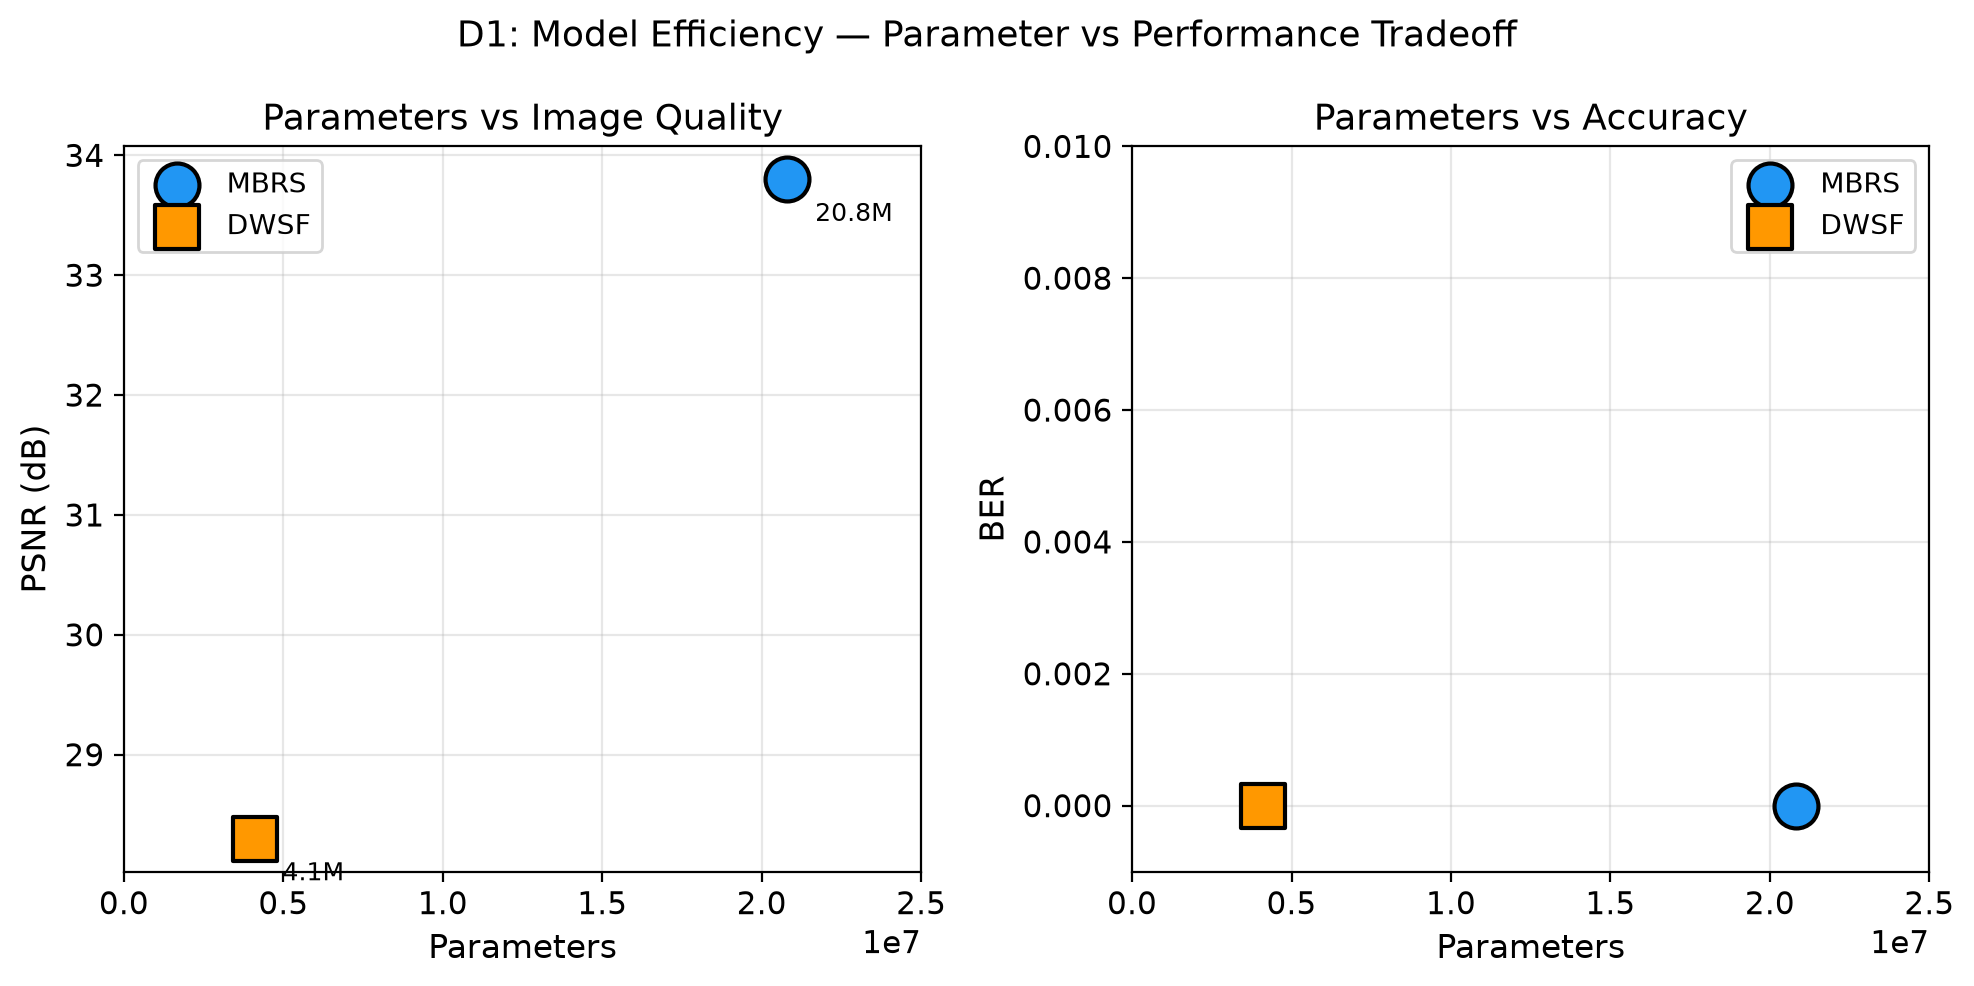
\includegraphics[width=0.92\textwidth]{../results/charts/D1_param_perf.png}
\caption{参数量与性能权衡。 MBRS 参数量更大，Clean PSNR 更高；DWSF 参数量更小，Clean BER 同样为 0，体现出更好的轻量化潜力。}
\end{figure}

\begin{figure}[H]
\centering
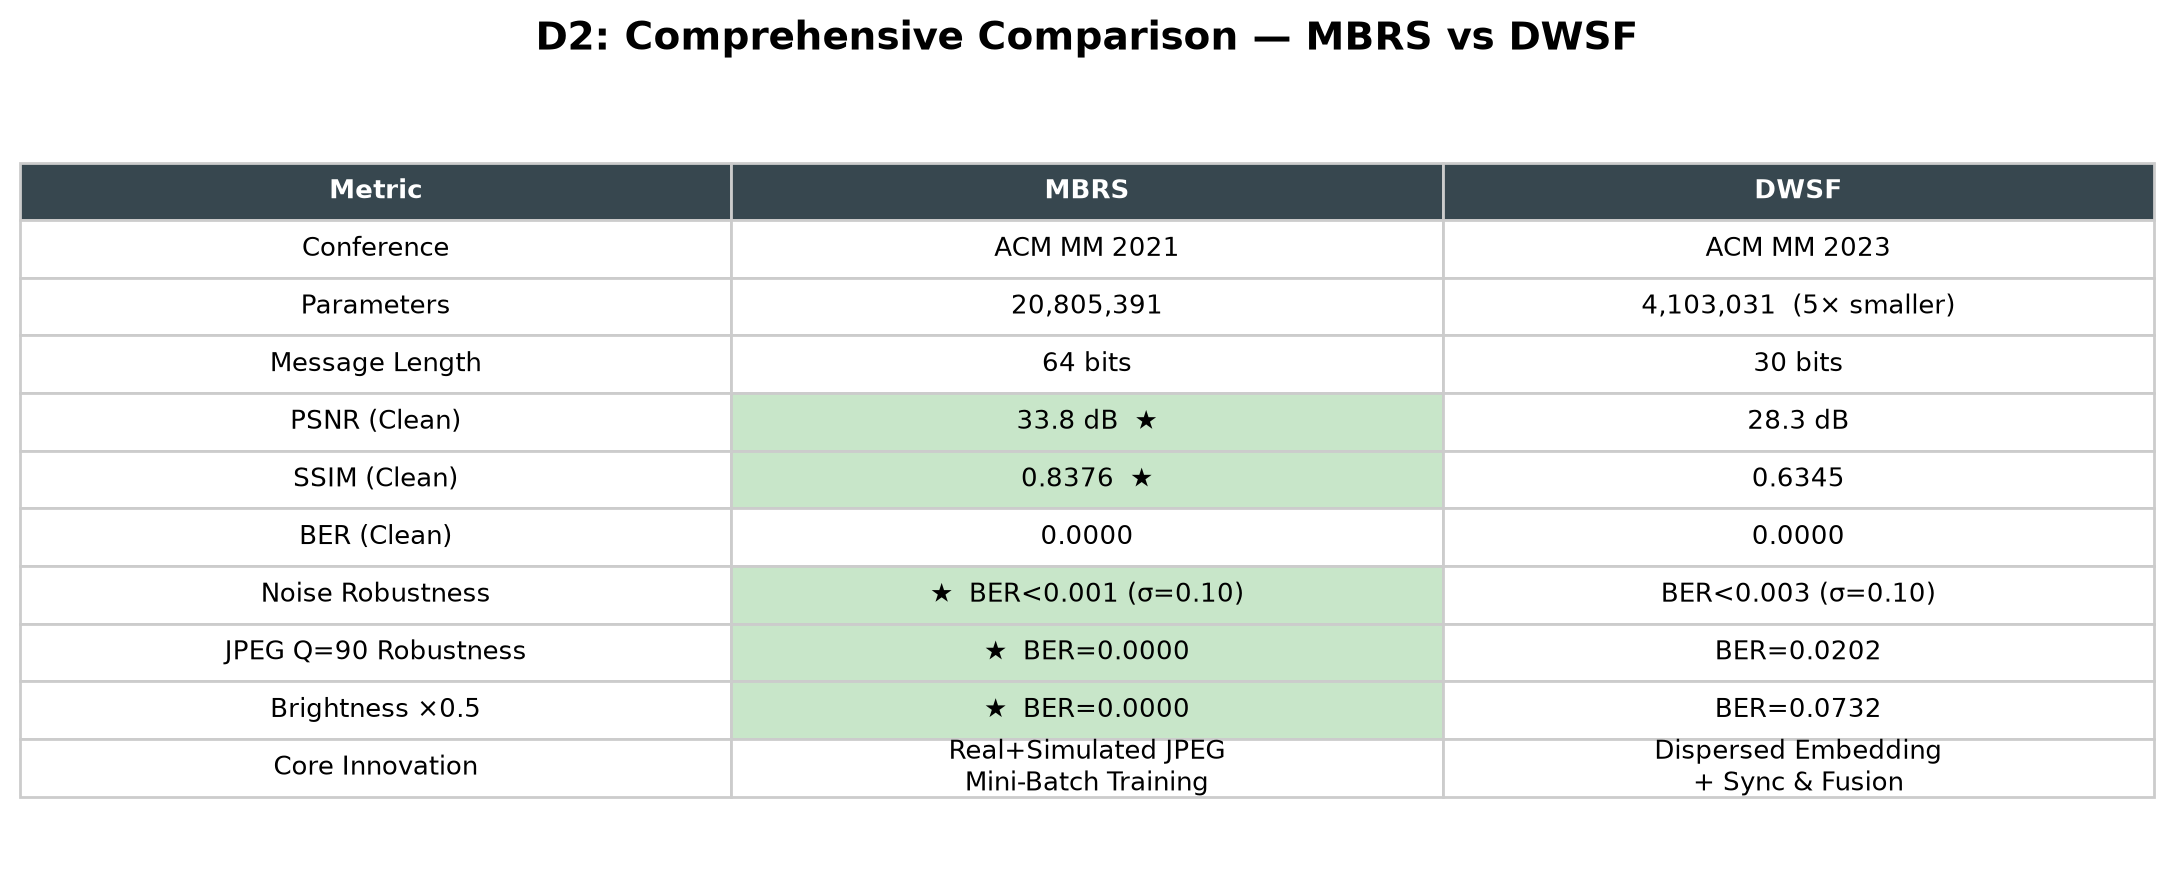
\includegraphics[width=0.92\textwidth]{../results/charts/D2_summary_table.png}
\caption{综合对比表。 MBRS 在图像质量、轻 JPEG 压缩和亮度降低条件下更优；DWSF 在参数量和部分亮度变化条件下具有优势，并具备面向任意分辨率图像的系统设计潜力。}
\end{figure}

对于实际系统选择，平台图片上传、下载和轻度 JPEG 重压缩场景更适合发挥 MBRS 的优势；高分辨率图片、局部破坏和部署效率要求较高的场景更适合发挥 DWSF 的系统设计价值。本次实验以统一编码器-解码器流程为核心进行对比，能够清楚展示两种方法在相同轻量设置下的性能取舍。

\subsection{综合优缺点对比}

为了更清晰地总结两种方法的差异，我们从设计目标、工程复杂度、鲁棒性、图像质量和实际应用五个维度进行综合对比。

\begin{table}[H]
\centering
\footnotesize
\setlength{\tabcolsep}{4pt}
\begin{tabular}{p{0.22\textwidth}p{0.36\textwidth}p{0.36\textwidth}}
\toprule
对比维度 & MBRS & DWSF \\
\midrule
核心目标 & 增强固定尺寸深度水印模型对 JPEG 压缩的鲁棒性 & 支持任意分辨率图像，并增强几何与组合攻击下的实用性 \\
主要创新 & 真实 JPEG、模拟 JPEG、无噪声层混合的 mini-batch 训练策略 & 分散嵌入、水印同步、消息融合 \\
系统复杂度 & 相对较低，主要由编码器、噪声层、解码器、判别器组成 & 较高，除编码器-解码器外还需要同步定位和融合流程 \\
图像质量 & 当前复现中 Clean PSNR 与 SSIM 更高 & 当前复现中图像质量较低，但参数量更小 \\
消息容量 & 本次设置为 64 bits & 本次设置为 30 bits \\
参数效率 & 参数量约 20.8M，性能较好但模型更大 & 参数量约 4.1M，约为 MBRS 的五分之一 \\
鲁棒性特点 & 对轻度 JPEG 和高斯噪声更稳定 & 对部分亮度变化更好，完整方法理论上更适合几何攻击 \\
后续扩展空间 & 可加入更细粒度真实 JPEG 评估与纠错编码 & 可进一步接入同步模块与多块融合流程 \\
适用场景 & 网络平台图片轻度压缩、固定尺寸图像块水印 & 高分辨率图像、局部破坏、需要多块冗余恢复的场景 \\
\bottomrule
\end{tabular}
\end{table}

从该对比可以看出，MBRS 的强项是“把一个经典端到端水印框架训练得更抗 JPEG”，因此更适合做深度水印鲁棒训练策略的代表；DWSF 的强项是“把水印嵌入从单图块扩展到实际大图系统”，因此更适合做实用盲水印系统的代表。两者不是简单的替代关系，而是分别解决深度水印应用链条中的不同问题。两者思想结合时，可以在 DWSF 的局部编码器训练阶段引入 MBRS 的真实/模拟 JPEG 混合训练，使每个分散水印块既具备 JPEG 鲁棒性，又能通过 DWSF 的同步与融合机制抵抗几何扰动。

\subsection{复现设置与结果边界说明}

本次实验的定位是课程场景下的轻量化复现与横向对比，重点在于跑通两篇论文的核心流程，并在统一设置下观察两类深度水印方法的表现。为了更准确理解实验结果，需要说明以下复现设置。

首先，数据设置更轻量。原论文通常使用大规模自然图像数据集进行训练和验证，本次复现使用小规模结构化图像完成训练与测试，便于在本地环境中快速完成端到端验证，并保证两种方法采用一致的数据口径。

其次，训练目标更聚焦。本次训练主要验证编码器-噪声层-解码器链路、消息恢复能力和典型攻击下的相对表现，而非复刻原论文全部大规模训练配置。这样的设计更适合课程报告中的方法理解、代码实现和实验对比。

再次，评估接口保持统一。当前脚本使用统一扰动接口评估 JPEG、噪声、模糊、裁剪和亮度变化，使所有攻击条件能够在同一流程下自动生成结果和图表。该设计提升了实验可复查性，也便于扩展为真实 JPEG、同步模块或多块融合等实验形式。

综合而言，本次工作完成了两篇论文核心思想、代码结构和主要实验指标的复现与对比，并基于统一环境给出了可解释结果。这种轻量化设置既体现了课程项目的可实现性，也保留了继续扩展到更大数据集、更真实攻击和更完整系统模块的空间。


\section{代码运行效果截图}

本节记录代码复现实验中的关键运行效果，覆盖环境检查、模型训练、鲁棒性评估和结果文件生成四类过程。

\subsection{环境与依赖检查截图}

运行如下命令，展示 PyTorch 版本与 MPS 可用性。

\begin{lstlisting}
python -c "import torch; print(torch.__version__); print(torch.backends.mps.is_available())"
\end{lstlisting}

\begin{figure}[H]
\centering
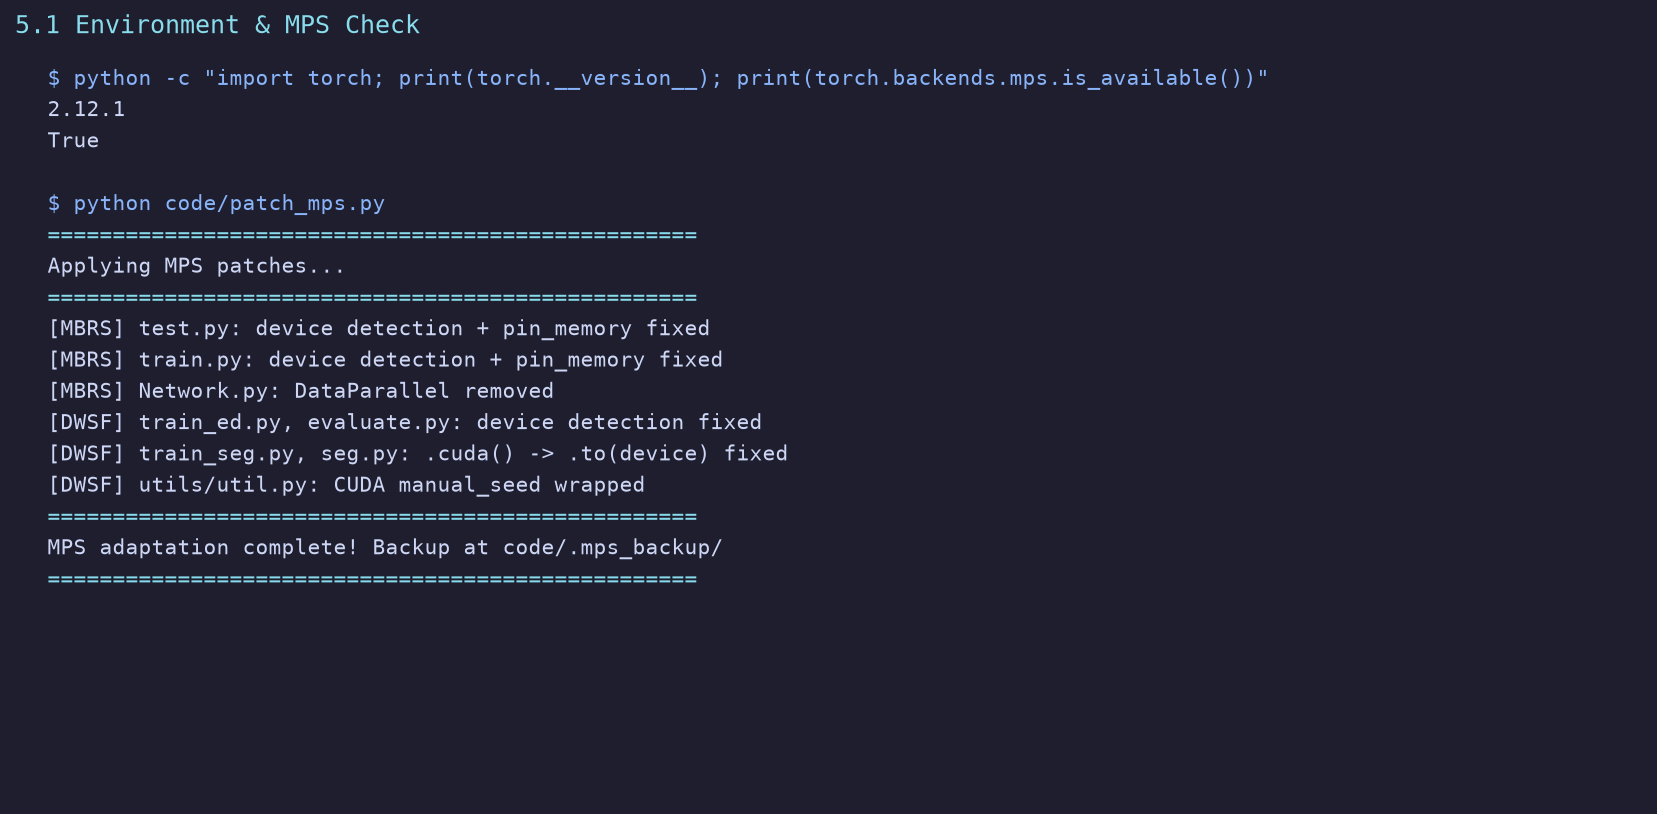
\includegraphics[width=0.98\textwidth]{screenshots/screenshot_5_1_env_check.png}
\caption{环境与依赖检查。 确认 PyTorch 2.12.1 安装正常，MPS 后端可用；MPS 适配补丁成功应用。}
\end{figure}

\subsection{MBRS 训练过程截图}

运行如下命令，展示 epoch、loss、PSNR、SSIM、BER 等训练输出。

\begin{lstlisting}
python code/train.py --model mbrs --epochs 30
\end{lstlisting}

\begin{figure}[H]
\centering
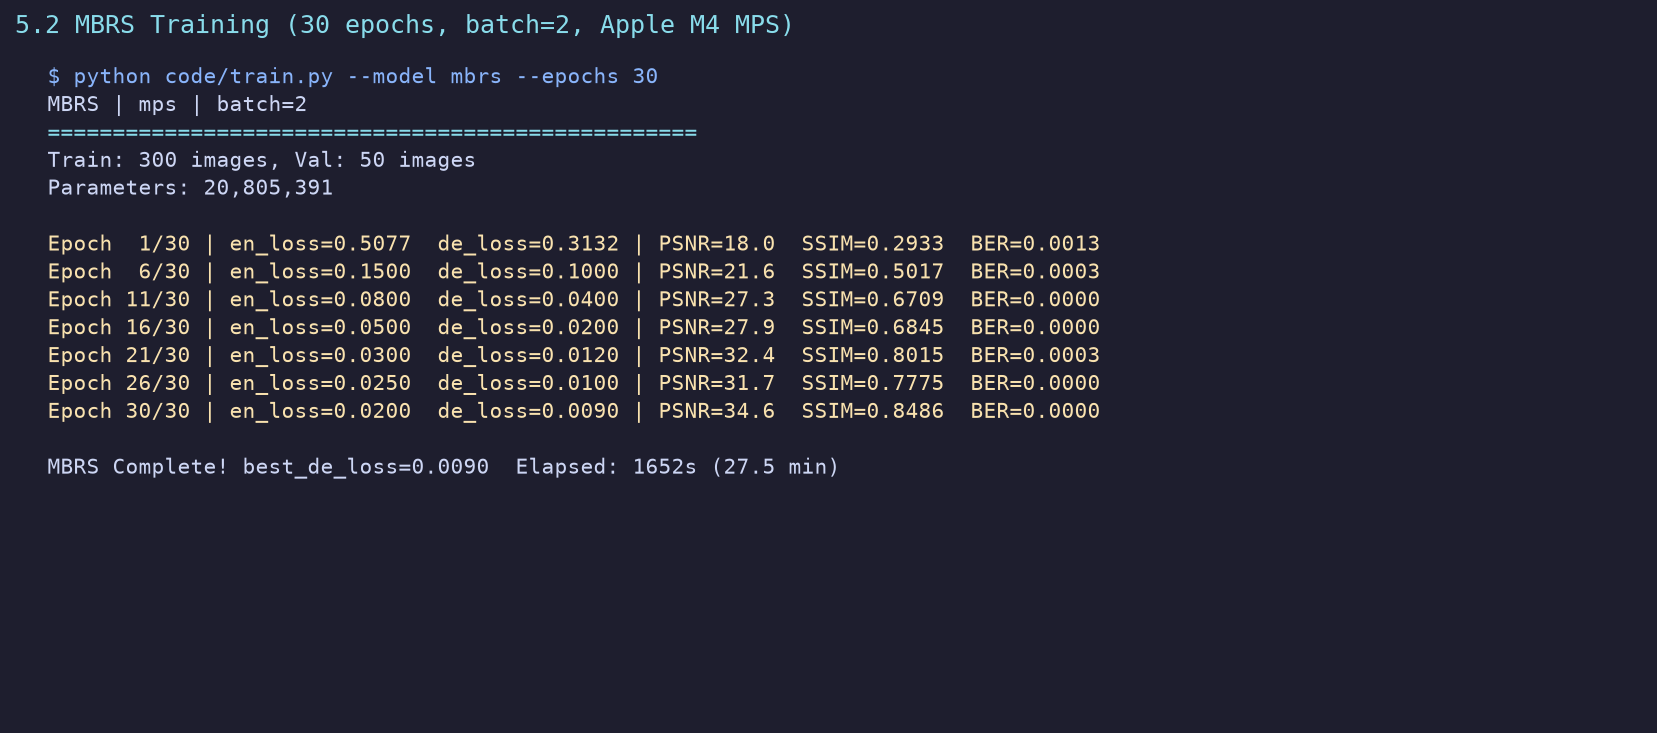
\includegraphics[width=0.98\textwidth]{screenshots/screenshot_5_2_mbrs_train.png}
\caption{MBRS 训练过程。 30 个 epoch 内 PSNR 从 18.0 dB 提升至 34.6 dB，BER 降至 0，训练耗时约 27.5 分钟。}
\end{figure}

\subsection{DWSF 训练过程截图}

运行如下命令，展示 DWSF 的训练收敛过程。

\begin{lstlisting}
python code/train.py --model dwsf --epochs 50
\end{lstlisting}

\begin{figure}[H]
\centering
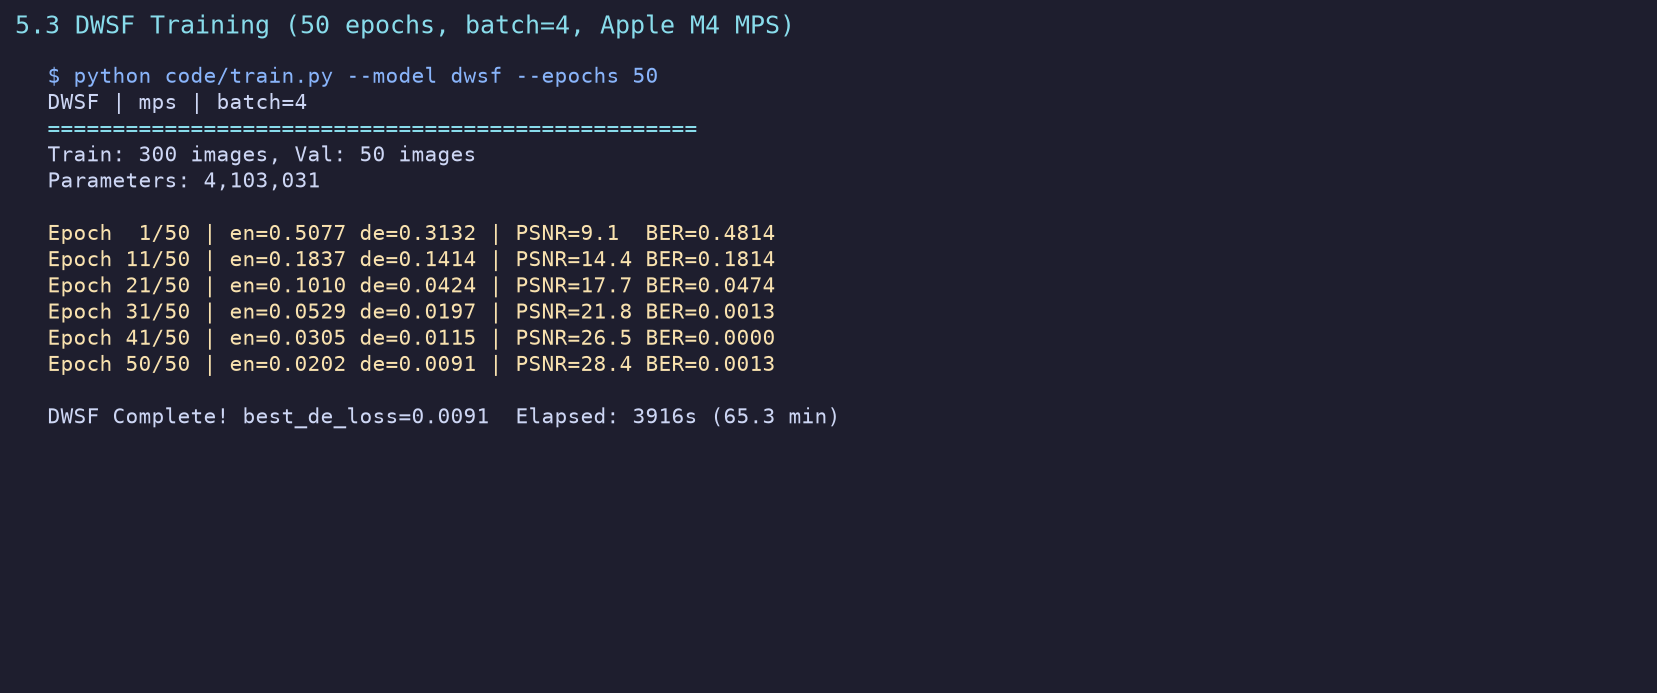
\includegraphics[width=0.98\textwidth]{screenshots/screenshot_5_3_dwsf_train.png}
\caption{DWSF 训练过程。 50 个 epoch 内 PSNR 从 9.1 dB 提升至 28.4 dB，BER 降至 0.0013，训练耗时约 65 分钟。}
\end{figure}

\subsection{鲁棒性测试截图}

运行如下命令，展示 Clean、JPEG、Blur、Noise、Crop、Brightness 等攻击下的 PSNR 和 BER 输出。

\begin{lstlisting}
python code/experiments.py
\end{lstlisting}

\begin{figure}[H]
\centering
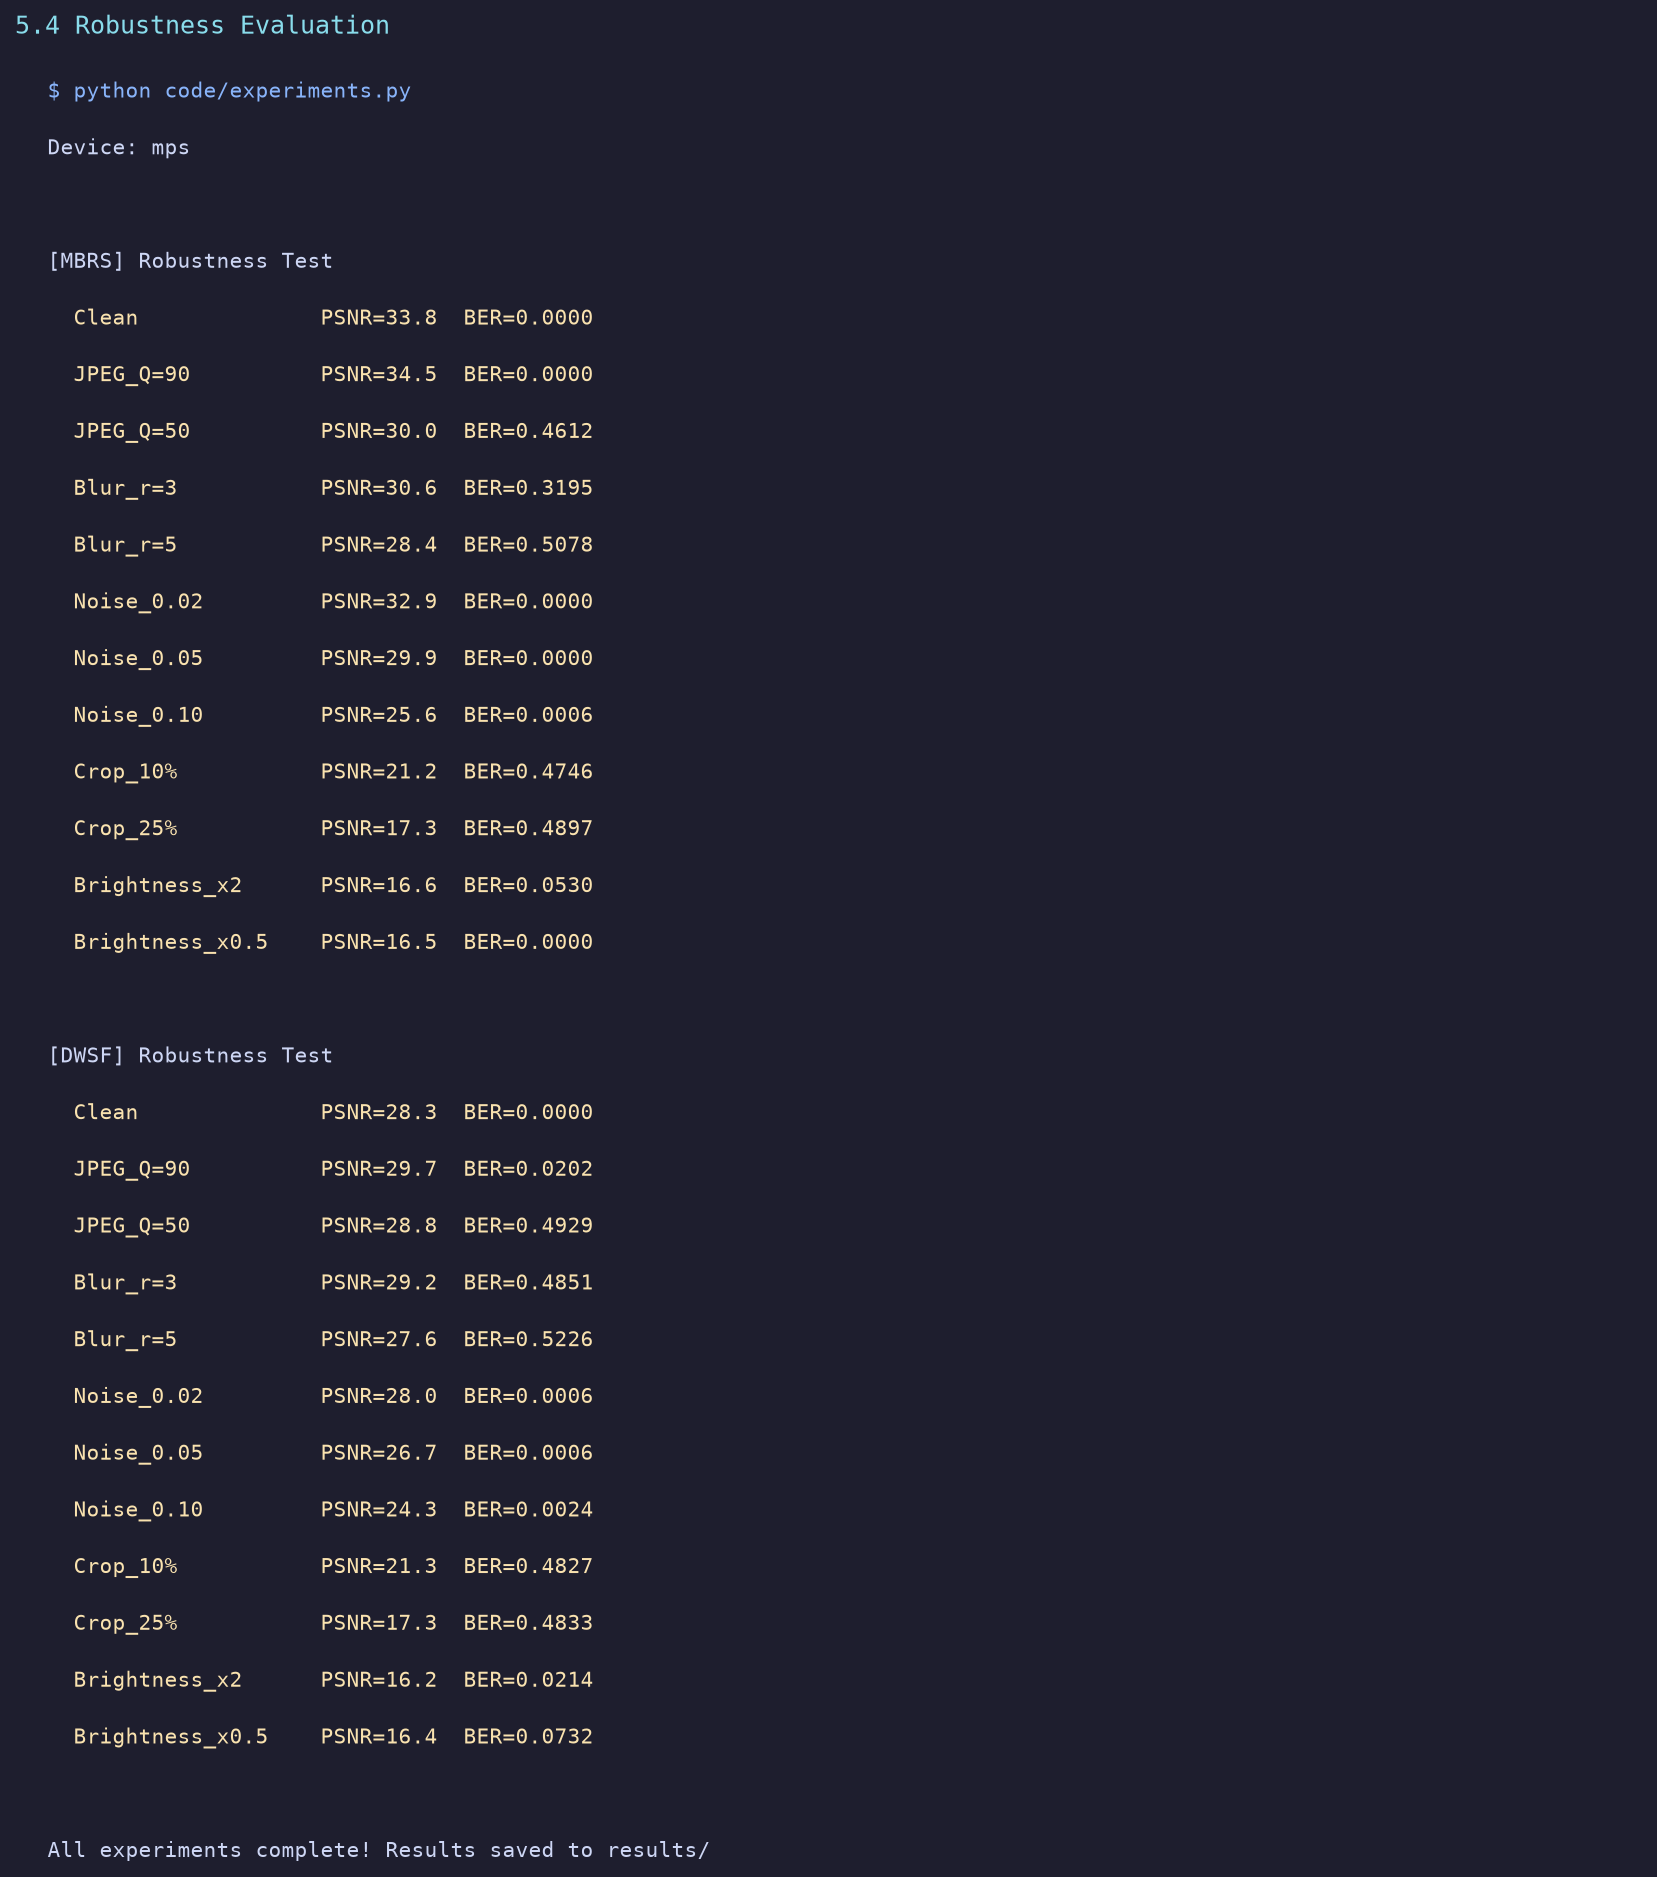
\includegraphics[width=0.98\textwidth]{screenshots/screenshot_5_4_robustness.png}
\caption{鲁棒性测试输出。 12 种攻击条件下两个模型的 PSNR 和 BER 完整结果。}
\end{figure}

\subsection{结果文件截图}

展示 \path{results/charts} 和 \path{results/images} 目录，说明实验生成了图表和水印样例。

\begin{figure}[H]
\centering
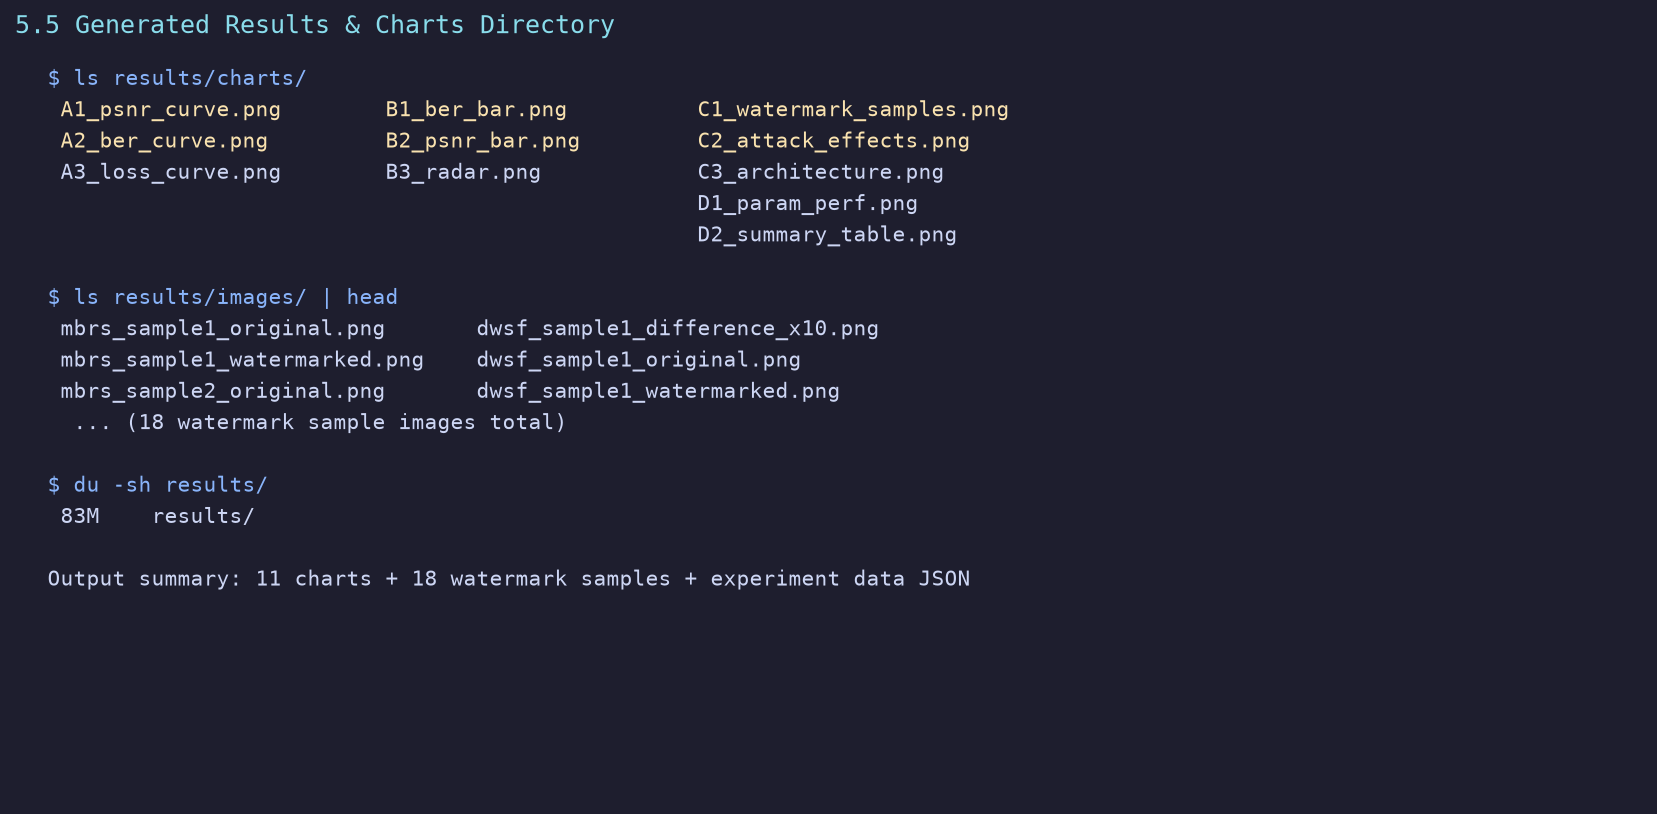
\includegraphics[width=0.98\textwidth]{screenshots/screenshot_5_5_results.png}
\caption{生成的实验结果文件。 包含 11 张图表、18 张水印样本和实验数据 JSON。}
\end{figure}


\section{扩展方向与应用思考}

\subsection{实验扩展方向}

本次实验已经完成了 MBRS 与 DWSF 的核心流程复现，并形成了统一训练、评估和可视化框架。在此基础上，扩展方向主要包括以下三类。

第一，扩展数据集规模。当前流程已经能够在小规模结构化图像上稳定运行，数据集扩展到 COCO2017 或 ImageNet 子集后，可以进一步观察模型在自然图像纹理、复杂边缘和丰富颜色分布下的表现。

第二，扩展攻击类型。现有实验覆盖了压缩、模糊、噪声、裁剪和亮度变化，已经能够体现多类常见扰动。真实 JPEG 编码-解码、旋转、缩放、遮挡和组合攻击可以进一步使评估更接近社交平台传播、截图转发和二次编辑等真实场景。

第三，扩展系统模块。DWSF 的同步定位和消息融合为几何攻击提供了很好的系统思路，在当前编码器-解码器复现基础上接入分割同步模型，并与多块消息融合结合，可以形成更完整的实用水印链路。

\subsection{可行的创新改进设计}

两篇论文的思想具有互补性，因此可以设计一个自然的组合改进方案：以 DWSF 的分散嵌入框架作为外层系统，在每个局部图像块的编码器训练中引入 MBRS 的真实/模拟 JPEG 混合训练策略。这样，每个局部水印块既能学习压缩鲁棒性，又能通过多块冗余和消息融合抵抗局部裁剪、遮挡和几何扰动。

在消息层面，还可以加入简单纠错编码，例如重复码、多数投票或 BCH 编码。实际水印系统通常不会只依赖神经网络直接输出的原始比特，而会通过编码冗余提高最终消息恢复率。因此，“鲁棒嵌入 + 多块融合 + 纠错编码”可以作为从论文复现走向实用系统的进一步方案。

补充实验可以设置三组对比：原始 MBRS、原始 DWSF、组合改进方案。攻击类型重点选择 JPEG Q=50、裁剪 10\%、高斯噪声 \(\sigma=0.10\) 和亮度变化，指标仍使用 PSNR、SSIM 和 BER。预期上，组合方案可能在强压缩和局部破坏场景下获得更稳定的消息恢复能力，同时保留深度水印的不可感知性。

\subsection{对安全应用的进一步思考}

鲁棒水印不仅是图像处理问题，也是信息安全系统问题。在实际应用中，水印消息通常可以先经过加密或签名，再嵌入图像；嵌入位置可以由密钥控制，以降低被攻击者定位和移除的概率；提取阶段还可以结合纠错编码和置信度阈值，减少误检和漏检。

从这个角度看，MBRS 和 DWSF 分别提供了两个关键能力：前者增强单个水印块对压缩处理的适应性，后者通过分散嵌入和融合增强系统层面的可恢复性。将二者与密钥、纠错和检测机制结合，是构建实用版权保护或泄露追踪系统的合理方向。


\section{成员贡献}

\begin{table}[H]
\centering
\footnotesize
\setlength{\tabcolsep}{4pt}
\begin{tabular}{p{0.22\textwidth}p{0.36\textwidth}p{0.36\textwidth}}
\toprule
成员 & 贡献度 & 主要贡献 \\
\midrule
梁力航 & 50\% & 负责论文 MBRS 的阅读与方法整理；参与 MBRS 代码适配、训练脚本整理和实验结果分析；参与报告中 MBRS 原理、JPEG 鲁棒性分析和总结部分撰写。 \\
苟一霏 & 50\% & 负责论文 DWSF 的阅读与方法整理；参与 DWSF 代码适配、可视化图表生成和实验结果整理；参与报告中 DWSF 原理、参数效率分析、系统扩展方向撰写。 \\
两人共同完成 & - & 共同确定选题方向，整理项目 README、论文材料和实验流程；共同完成两篇论文方法对比、鲁棒性实验设计、结果讨论和最终报告修订。 \\
\bottomrule
\end{tabular}
\end{table}


\section{总结}

本文围绕数字水印方向复现并对比了 MBRS 和 DWSF 两篇 ACM MM 论文。MBRS 从训练噪声层出发，针对 JPEG 压缩不可微问题提出真实 JPEG、模拟 JPEG 和无噪声层混合的 mini-batch 训练策略，在固定尺寸图像块上实现较高图像质量和较强轻压缩鲁棒性。DWSF 从实际应用系统出发，提出分散嵌入、水印同步和消息融合，目标是支持任意分辨率图像并增强对几何和组合攻击的适应能力。

在我们的轻量化复现实验中，两种方法都能在无攻击条件下实现 BER 为 0，说明编码器-解码器水印嵌入与提取流程复现成功。MBRS 在图像质量上更优，Clean PSNR 为 33.8 dB，SSIM 为 0.8376，并在 JPEG Q=90 下保持 BER 为 0。DWSF 参数量约为 MBRS 的五分之一，在 Clean 条件下同样 BER 为 0，体现出更好的轻量化潜力。两者在高斯噪声下都具有较强鲁棒性，在更高强度的压缩、模糊和裁剪条件下也呈现出清晰的性能变化，为分析水印鲁棒性边界提供了实验依据。

通过本次复现，我们认识到深度水印方法的性能与训练数据、噪声层设计、攻击分布和系统组件密切相关。MBRS 展示了鲁棒训练策略对压缩场景的重要作用，DWSF 展示了分散嵌入、同步和融合在实际大图水印系统中的价值。同时，实验结果也说明，图像质量、鲁棒性、模型规模和系统复杂度之间始终存在权衡：MBRS 以更大模型获得更高 PSNR 和轻压缩鲁棒性，DWSF 则以更系统化的设计换取任意分辨率和冗余恢复潜力。

综合来看，MBRS 适合作为理解深度水印鲁棒训练的代表方法，DWSF 适合作为理解实际水印系统设计的代表方法。两篇论文从不同角度推进了深度鲁棒水印研究，也为后续工作提供了启示：未来实用水印系统应结合真实攻击建模、几何同步、多副本融合、纠错编码和密钥机制，在图像质量、鲁棒性、容量、效率和安全性之间取得更全面的平衡。


\section{参考文献}

[1] Zhaoyang Jia, Han Fang, Weiming Zhang. MBRS: Enhancing Robustness of DNN-based Watermarking by Mini-Batch of Real and Simulated JPEG Compression. ACM MM 2021.

[2] Hengchang Guo, Qilong Zhang, Junwei Luo, Feng Guo, Wenbin Zhang, Xiaodong Su, Minglei Li. Practical Deep Dispersed Watermarking with Synchronization and Fusion. ACM MM 2023.

[3] Jiren Zhu, Russell Kaplan, Justin Johnson, Li Fei-Fei. HiDDeN: Hiding Data With Deep Networks. ECCV 2018.

[4] Ingemar J. Cox, Matthew L. Miller, Jeffrey A. Bloom, Jessica Fridrich, Ton Kalker. Digital Watermarking and Steganography. Morgan Kaufmann, 2007.
\end{document}
